\documentclass[10pt]{article}
\usepackage{commands}
\usepackage[sc]{mathpazo}

\begin{document}
\begin{tcolorbox}
  \begin{center}
  \begin{Large}
    \textbf{MATH 320/321 (Real Analysis) Notes} \\
    \vspace{5pt}
  \end{Large}
  \begin{large}
        Rio Weil \\
\vspace{5pt}
    \emph{This document was typeset on \today}
  \end{large}
  \end{center}
\end{tcolorbox}

\begin{center}
  \textbf{Introduction:}
  
  This set of notes is transcribed from UBC's MATH 320/321 (Real Variables I/II) sequence. The course covers the first 9 chapters of Rudin's ``Principles of Mathematical Analysis'' with occasional omissions \& additions. The numbering of the definitions/theorems/examples will follow that used in Rudin for convenience. The structure of these notes is such that they are split into main text (the boxed elements) and side text (everything else). It is possible to solely read the main text for all of the material, but the additional discussion provided by the side text may be useful. If any errors are found in the notes, feel free to email me at \texttt{ryoweil6@student.ubc.ca}.
\end{center}

\addtocontents{toc}{\protect\hypertarget{toc}{}}
\tableofcontents

\newpage

\section{The Real and Complex Number Systems}
\subsection{The Naturals, Integers, and Rationals}
We begin by a review of number systems which are already familiar.

\begin{ndef}{The Natural Numbers}
    The \textbf{Naturals}, denoted by $\NN$, is the set $\set{1, 2, 3, \ldots}$.
\end{ndef}

\noindent For $x, y, \in \NN$, we have that $x + y \in \NN$ and $xy \in \NN$, so the naturals are closed under addition and multiplication. However, we note that it is not closed under subtraction; take for example $2 - 4 = -2 \notin \NN$.

\begin{ndef}{The Integers}
    The \textbf{Integers}, denoted by $\ZZ$, is the set $\set{\ldots, -3, -2, -1, 0, 1, 2, 3, \ldots}$.
\end{ndef}

\noindent The integers are closed under addition, multiplication, and subtraction. However, it is not closed under division; for example, $1/2 \notin \ZZ$. 

\begin{ndef}{The Rationals (informal)}
    The \textbf{Rationals}, denoted by $\QQ$, can be defined as $\set{\frac{m}{n}: m \in \ZZ, n \in \NN}$, where $\frac{m_1}{n_1}$ and $\frac{m_2}{n_2}$ are identified if $m_1n_2 = m_2n_1$.
\end{ndef}

\noindent We note that unlike the naturals/integers, the rationals do not have as obvious of a denumeration. This above is a good definition if we already have the same rigorous idea of what a rational number is in our mind; i.e. it works because we have a shared preconceived understanding of a rational number.

If this is not the case, it may help to define the rational numbers more rigorously/formally (even if the definition may be slightly harder to parse). As a second attempt at a definition, we can say that $\QQ$ is the set of ordered pairs $\set{(m, n): m \in \ZZ, n \in \NN}$. However, this is not quite enough as we need a notion of equivalence between two rational numbers (e.g. $(1, 2) = (2, 4)$). Hence, a complete and rigorous definition would be:

\begin{ndef}{The Rationals (formal)}
    The \textbf{Rationals}, denoted by $\QQ$, is the set $\set{(m, n): m \in \ZZ, n \in \NN}/\sim$ where $(m_1, n_1) \sim (m_2, n_2)$ if $m_1n_2 = m_2n_1$.
\end{ndef}
\noindent Under the formal definition, the rationals are a set of equivalence classes of ordered pairs, under the equivalence relation $\sim$. We note that the rationals are closed under addition, subtraction, multiplication, and division.

This formal definition might be slightly harder to parse, so it might be useful to consider an example with a similar flavour. Consider the set $X = \set{m \in \ZZ}/\sim$ such that $m_1 \sim m_2$ if $m_1 - m_2$ is divisible by 12. This is "clock arithmetic", with equivalence classes $[0], [1], [2], \ldots$ for each hour on an analog clock. A fun side note: If instead of 12 we picked a prime number, we would get a field (we will discuss what this is in a later lecture)!

Note that under this definition, $(1, 2)$ and $(2, 4)$ are different representations of the same rational number. With this definition, we would define addition such that $(m_1, n_1) + (m_2, n_2) = (m_1n_2 + m_2n_1, n_1n_2)$. Note that $(2m_1, 2n_2) + (m_2, n_2) = (2m_1n_2 + 2m_2n_1, 2n_1n_2)$ and we can identify $(m_1n_2 + m_2n_1, n_1n_2)$ with $(2m_1n_2 + 2m_2n_1, 2n_1n_2)$. If we choose different representations when we do addition, we might get a different representation in our result, but it will represent the same rational number regardless of the choice of representations we originally chose to do the addition. 

A natural question then becomes if the rationals are sufficient for doing all of real analysis. Certainly, it seems as we have a number system that is closed under all our basic arithmetic operations; but is this enough? For example, are we able to take limits just using the rationals? The answer turns out to be no (they are insufficient!) and the following example will serve as one illustration of this fact. 

\begin{example}{Incompleteness of the Rationals}{1.1a}
    There exists no $p \in \QQ$ such that $p^2 = 2$.
\end{example}
\noindent We proceed via proof by contradiction. Recall in that these types of proof, we start with a certain wrong assumption, follow a correct/true line of reasoning, reach an eventual absurdity, and therefore conclude that the original assumption was mistaken. 
\begin{nproof}
    Let us then suppose for the contradiction that there exists $p = \frac{m}{n}$ with $p^2 = 2$. We then have that not both $m, n$ are even, and hence at least one is odd. Then, we have that $2 = p^2 = \frac{m^2}{n^2}$ and hence $m^2 = 2n^2$, so $m^2$ is even, implying $m$ is even. So, let us write $m = 2k$ for $k \in \ZZ$. Then, $(2k)^2 = 4k^2 = 2n^2$, and hence $2k^2 = n^2$. Therefore, $n^2$ is even and hence $n$ is even. $m$ and $n$ are therefore both even, a contradiction. We conclude that no such $p$ exists. \qed
\end{nproof}
\noindent Why can we conclude that not both $m, n$ are even in the above proof? This is the case as if $m, n$ we both even, then we could write $m = 2m'$, $n = 2n'$ for some $m', n'$, and then $p = \frac{m}{n} = \frac{2m'}{2n'} = \frac{m'}{n'}$ which we can continue until either the numerator or denominator is odd. A natural question to consider is how to prove that this process of reducing fractions will eventually conclude. The resolution is to invoke the fundamental theorem of arithmetic, and write $m, n$ in terms of their unique prime factorization. We are then able to cancel out factors of 2 from the numerator/denominator until at least one is odd.

We note that this example leads us to conclude that the rationals have certain "holes" in them. This is concerning, as there are sequences of rational numbers that tend to $\sqrt{2}$. Conversely, its not as concerning that there is no rational number $x$ such that $x^2 = -1$, as there is no such sequence of rational numbers that is "close to" $i$ (note that both $\sqrt{2}$ and $i$ have not yet been defined, but this will come shortly).

\setcounter{rudin}{0}

\begin{example}{Incompleteness of the Rationals}{1.1b}
    Let $A = \set{p \in \QQ: p > 0, p^2 < 2}$, and $B = \set{p \in \QQ: p > 0, p^2 > 2}$. Then, $\forall p \in A, \exists q \in A$ such that $p < q$, and $\forall p \in B, \exists q \in B$ such that $q < p$. 
\end{example}
\begin{figure}[htbp]
    \centering
    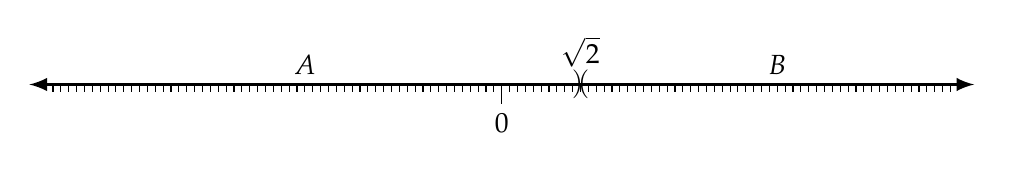
\begin{tikzpicture}
        \draw[latex-latex, very thick] (-6, 0) -- (6,0) node[anchor=south] {$\QQ$};
        \draw[] (0, 0) -- (0, -0.25) node[anchor=north] {0};
        \foreach \i in {-5.7,-5.6,...,5.7}{ 
        \draw[] (\i,0) -- (\i,-0.1);
        }
        \draw[] (1,0.1) node[anchor=south] {$\sqrt{2}$};
        \draw[] (0.96,0) node[] {$)$};
        \draw[] (1.04,0) node[] {$($};
        \draw[] (-2.5, 0) node[anchor=south] {$A$};
        \draw[] (3.5, 0) node[anchor=south] {$B$};
    \end{tikzpicture}
    \caption{Visualization of sets $A$ and $B$. We note that $\sqrt{2}$ has not been defined in our formalism yet, but from our prior mathematical intuition it would be what goes in the "hole" of the rationals.}
    \label{fig1}
\end{figure}

\noindent For the proof of this statement, we consider playing a 2 person game. One person is $\forall$, one person is $\exists$, and we consider if one person has a winning strategy. $\forall$ goes first, and then $\exists$ goes next, having seen the choice that $\forall$ has made. Then, we check if indeed $p < q$. If $p < q$, then $\exists$ wins. If $p \not< q$, then $\forall$ wins. 

\begin{nproof}
    Let $p \in A$. Then, let $q = \frac{2p + 2}{2 + p}$. Since $p \in \QQ$, it follows that $2p + 2 \in \QQ$ and $2 + p \in \QQ$ so $q \in \QQ$. Furthermore, we have that $2p + 2 > 0$ and $2 + p > 0$, so $q > 0$. We also have that:
    \[q^2 = \frac{(2p+2)^2}{(2+p)^2} = 2 + \frac{2(p^2 - 2)}{(p+2)^2} < 2\]
    Where the inequality follows from the fact that $p^2 < 2$ and hence $(p^2 - 2) < 0$. It therefore follows that $q \in A$. Finally, we have that:
    \[q = p + \frac{2-p^2}{2+p} > p\]
    so $q > p$, completing the proof of the first part of the claim. The second part is left as an exercise (we note that the same $q$ can be used). \qed
\end{nproof}

\noindent The number $q = \frac{2p+ 2}{2 + p}$ seems to be pulled out of a hat, but actually comes from a fairly geometric picture (the secant method of approximating roots). Discussion on this topic can be found here: \\ \texttt{https://math.stackexchange.com/questions/141774/choice-of-q-in-baby-rudins-example-1-1}.

\subsection{Ordered Sets}
Over the next couple sections, we will be discussing certain properties of sets that will give us a better understanding of the real numbers, and allow us to construct them.

\setcounter{rudin}{4}

\begin{definition}{Order}{1.5}
    An \textbf{order} $<$ on a set $S$ is a relation with the following properties:
    \begin{enumerate}[(i)]
        \item For every pair $x, y \in S$, exactly one of $x < y$, $x = y$, or $y < x$ is true. 
        \item For $x, y, z \in S$, if $x < y$ and $y < z$, then $x < z$. 
    \end{enumerate}
    A point on notation; We note that $x > y$ means $y < x$, and $x \leq y$ means $x < y$ or $x = y$. 
\end{definition}

\begin{definition}{Ordered Sets}{1.6}
    An ordered set is a pair $(S, <)$. We may write just $S$ if the order can be inferred by the context.
\end{definition}
\noindent A familiar (and useful) set of examples is $S = \NN$ or $S = \ZZ$ or $S = \QQ$. For these three sets, we have that $x < y$ if $y-x$ is positive. For another example, consider the set $S$ of english words; then the order $<$ can be the dictionary/lexographic order. 

\begin{definition}{Upper \& Lower Bounds}{1.7}
    Let $S$ be an ordered set and $E \subset S$ (note that here, $E \subset S$ is a non-strict subset, and $E \subsetneq S$ is a strict subset). $E$ is \textbf{bounded above} if there exists an element $\beta \in S$ such that $\forall x \in E$, $x \leq \beta$. Any such $\beta$ is an \textbf{upper bound} of $E$. Similarly, we say that $E$ is \textbf{bounded below} if there exists an element $\alpha \in S$ such that $\forall x \in E$, $\alpha \leq x$. In this case, $\alpha$ is a \textbf{lower bound} of $E$.
\end{definition}
\noindent As an example, one can take $S = \QQ$, $E = A = \set{p \in \QQ: p > 0, p^2 > 2}$ (as in Example \ref{exam:1.1b}). Here, $E$ is bounded above, with $\beta = 2$ as one possible upper bound. to see this is the case, consider that if $p \in E$:
\[2 - p = \frac{4 - p^2}{2+p} > \frac{4-2}{2+p} > 0\]
\noindent However, if we take $S = A$, $E = A$, then $E$ is not bounded above as we saw in the example. There is no upper bound of $A$ in $A$. In general, this example reveals the subtle point that "the upper bound of a set" is ill-defined; we need to specify $E \subset S$. 

\subsection{The Least Upper Bound Property}
\begin{definition}{Least Upper Bound \& Greatest Lower Bound}{1.8}
    Let $S$ be an ordered set, and let $E \subset S$ with $E$ bounded above. If $\exists \alpha \in S$ such that:
    \begin{enumerate}[(i)]
        \item $\alpha$ is an upper bound for $E$
        \item If $\gamma < \alpha$, then $\gamma$ is not an upper bound for $E$
    \end{enumerate} 
    The $\alpha$ is the \textbf{least upper bound}, or \textbf{supermum} of $E$. This can be denoted as $\alpha = \sup(E)$. Analogously, the \textbf{greatest lower bound}, or \textbf{infimum} of E (denoted $\alpha = \inf(E)$) is an element $\alpha \in S$ (if it exists) such that:
    \begin{enumerate}[(i)]
        \item $\alpha$ is a lower bound for $E$
        \item If $\gamma > \alpha$, then $\gamma$ is not an upper bound of $E$. 
    \end{enumerate}
\end{definition}

\begin{ntheorem}{Uniqueness of supremum/infimum}
    If the supremum/infimum of $E \subset S$ exist, they are unique.
\end{ntheorem}
\begin{nproof}
        Let $E \subset S$. Suppose that there exist $\alpha_1, \alpha_2$ such that $\alpha_1 = \sup(E)$ and $\alpha_2 = \sup(E)$. If $\alpha_1 < \alpha_2$, as $\alpha_1$ is an upper bound of $E$, this contradicts the fact that $\alpha_2$ is the least upper bound of $E$. We reach an identical contradiction if $\alpha_2 < \alpha_1$. Therefore we conclude that $\alpha_1 = \alpha_2$ and the supremum of $E$ is unique (if it exists). The proof for the infimum is analogous. \qed
\end{nproof}

\begin{ntheorem}{Equivalence of maximum and supremum}
    If $E \subset S$ has a maximum element $\alpha$ (that is, an element such that $x < \alpha$ for all $x \in E$) then $\alpha = \sup(E)$. Similarly, if $E$ has a minimum element $\alpha$, then $\alpha = \inf(E)$. The proof is left as an exercise. 
\end{ntheorem}

\begin{comment}
\begin{nproof}
    Let $E \subset S$ and $\alpha = \max(E)$. By definition $\alpha$ is an upper bound of $E$, and if $x < \alpha$ for some $x \in E$ then $x$ is not an upper bound of $E$ as it is not greater than $\alpha \in E$. The claim follows (with an identical proof for the minimum). \qed
\end{nproof}
\end{comment}

\begin{example}{}{1.9}
    \begin{enumerate}
        \item Consider again the sets $A, B \subset \QQ$ from example \ref{exam:1.1b}. $A$ is bounded above by any element in $B$, and the upper bounds of $A$ are exactly the elements of $B$. Since $B$ has no smallest member, $A$ does not have a least upper bound in $\QQ$.
        \item Let $E_1, E_2 \subset \QQ$ such that $E_1 = \set{r: \QQ, r < 0}$ and $E_2 = \set{r: \QQ, r \leq 0}$. Then $\sup(E_1) = \sup(E_2) = 0$. Note that this example shows that the supremum can either be contained or not contained in the set; $0 \notin E_1$ but $0 \in E_2$. 
        \item Let $E \subset \QQ$ such that $E = \set{\frac{1}{n}: n \in \NN}$. Then $\sup(E) = 1$ and $\inf(E) = 0$. This is proven below. 
    \end{enumerate}
\end{example}
\begin{nproof}
    $\sup(E) = 1$ immediately follows from the equivalence of the maximum and supremum as proven above. To see that $\inf(E) = 0$, first note that $0$ is a lower bound for $E$ as all of the elements of $E$ are positive. To see that it is the lower bound, take any $x > 0$. Then, we have that for any $n > \frac{1}{x}$, $\frac{1}{n} < x$ and hence $x$ is not an upper bound of $E$. This proves the claim. \qed
\end{nproof}

\begin{definition}{The LUB/GUB Property}{1.10}
    An ordered set $S$ has the \textbf{least upper bound property} if for every $E \subset S$, if $E \neq \emptyset$ and $E$ is bounded above, then $E$ has a least upper bound (that is, $\sup(E)$ exists in $S$). Similarly, an ordered set $S$ has the \textbf{greatest lower bound property} if for every $E \subset S$, if $E \neq \emptyset$ and $E$ is bounded below, then $E$ has a greatest lower bound.
\end{definition}
\noindent We will show in the next theorem that these properties are actually equivalent; before then, we briefly consider two examples.
\begin{nexample}{$\ZZ$ and $\QQ$}
    $\ZZ$ has the least upper bound property, while $\QQ$ does not. 
\end{nexample}
\begin{nproof}
    For the first claim, consider any nonempty $E \subset \ZZ$ that is bounded above. Choose any $x \in E$. Since $\ZZ$ is bounded above, there exist finitely many elements that are greater than $x$. Take the maximum of these finitely many elements. This maximum is also the maximum of $E$, so it is the supremum of $E$. Therefore $\ZZ$ has the LUB property as claimed.
    
    The second claim immediately follows from Example \ref{exam:1.9}(a). \qed
\end{nproof}

\begin{theorem}{Equivalence of LUB/GUB properties}{1.11}
    Let $S$ be an ordered set. Then $S$ has the LUB property if and only if it has the GUB property. 
\end{theorem}
\begin{nproof}
    $\boxed{\implies}$ Let $S$ be an ordered set with the LUB property. Let $E \subset S$ with $E \neq \emptyset$, with $E$ bounded below. Let $L = \set{x \in S: x\text{ is a lower bound of $E$.}}$. $L \neq \emptyset$ as $E$ is bounded below (and hence has at least one lower bound). If $y \in E$, then $y$ is an upper bound for $L$. Since $E$ is nonempty, $L$ is therefore bounded above. Since $S$ has the LUB property, then $\sup(L)$ must exist. Let us call this $\alpha$. Then, $\alpha \leq x\ \forall x \in E$ (as if $\gamma < \alpha$, then $\gamma$ is not an upper bound of $L$ and hence $\gamma \neq E$). Hence, $\alpha$ is a lower bound for $E$ and hence $\alpha \in L$. Since $\alpha = \sup(L)$ and $\alpha$ is an upper bound for $L$, we have that $\alpha \geq \gamma\ \forall \gamma \in L$. Thus, $\alpha = \inf(E)$. 

    $\boxed{\impliedby}$ Left as an exercise. \qed
\end{nproof}

\subsection{Fields and Ordered Fields}
\begin{definition}{Fields}{1.12}
    A field $F$ is a set with two binary operations, $+$ and $\cdot$ (addition and multiplication) such that the following axioms are satisfied:
    \begin{enumerate}[start=1, label={(A\arabic*):}]
    \item If $x, y \in F$, then $x + y \in F$. (Closure under addition)
    \item $x + y = y + x$ for all $x, y \in F$. (Commutativity of addition)
    \item $(x+y) + z = x + (y + z)$ for all $x, y, z \in F$. (Associativity of addition)
    \item $\exists 0 \in F$ such that $\forall x \in F$, $0 + x = x$. (Additive identity)
    \item $\forall x \in F$, $\exists y$ such that $x + y = 0$. We can denote $y = -x$. (Additive inverse)
    \end{enumerate}
    \begin{enumerate}[start=1, label={(M\arabic*):}]
        \item If $x, y \in F$, then $x\cdot y\in F$. (Closure under multiplication)
        \item $x \cdot y = y \cdot x$ for all $x, y \in F$.
        \item $(x\cdot y)\cdot z = x \cdot (y \cdot z)$ for all $x, y, z \in F$. (Associativity under multiplication)
        \item $\exists 1 \in F$ such that $1 \neq 0$ and $\forall x \in F$, $1 \cdot x = x$. (Multiplicative identity)
        \item $\forall x \in F$, exists $y \in F$ such that $x \cdot y = 1$. We can denote $y = \frac{1}{x}$. (Multiplicative inverse)
    \end{enumerate}
    (D): $x \cdot (y + z) = x \cdot y + x \cdot z$, $\forall x, y, z \in F$. (Distributive law)
\end{definition}
\noindent Note that A3/M3 show that $x + y + z$ and $x\cdot y\cdot z$ are well defined in a mathematical sense; however, associativity may not hold for computers that do math with finite precision! 
\begin{ntheorem}{Uniqueness of Identities and Inverses}
    The additive/multiplicative identities given by (A4)/(M4) and the additive/multiplicative inverses given by (A5)/(M5) are unique. 
\end{ntheorem}
\begin{nproof}
    Let $F$ be an ordered field. Suppose that there exist $0_1, 0_2 \in F$ such that $0_1 + x= x$ and $0_2 + x = x$ for all $x \in F$. We then have that:
    \begin{align*}
        0_1 + 0_2 &= 0_1 + 0_2
        \\ 0_1 + 0_2 &= 0_2 + 0_1 & \text{(A2)}
        \\ 0_2 &= 0_1 & \text{(Property of additive identity)}
    \end{align*}
    Which shows that the additive identity is unique. The remaining proofs are left as an exercise. \qed
\end{nproof}
\noindent Some easy (and familiar) consequences of the field axioms can be found in Rudin 1.14-1.16. Instead of repeating those here, we will discuss some examples. 

The rationals form a field (under the usual notions of addition/multiplication), but the integers do not, as there are no multiplicative inverses (e.g. there exists no integer $x \in \ZZ$ such that $2\cdot x = 1$). The simplest example of a field is $F = \set{0, 1}$, with the relations:
\begin{align*}
    0 + 0 = 0\quad 0\cdot0 = 1
    \\ 0 + 1 = 0 \quad 0 \cdot 1 = 0
    \\ 1 + 1 = 0 \quad 1 \cdot 1 = 1
\end{align*}
This field is often called $\mathbb{F}_2$ or $F_2$, and is useful in computer science (where bits can take on two states, 0 or 1). As a slight tangent, a byte (8 bits) can be considered an element of an 8-dimensional vector space over the field $\mathbb{F}_2$, where $+$ would be the XOR operator and $\cdot$ would be the AND operation. 

A generalization of the above example is $\mathbb{F}_p$ or $F_p$, for a prime number $p$. This field would consist of the elements $0, 1, \ldots, p-1$. The addition and multiplication are carried out mod $p$. An interesting result is that in general, finite fields must have cardinality of some prime power. 

Note that a field cannot have a single element; the field axioms (A4) and (M4) require the existence of distinct additive and multiplicative identities, which a singleton set cannot satisfy. 

Although algebra is not the focus of this course, it may be interesting to briefly think about sets with less structure than a field. We start by considering a group. 

\begin{ndef}{Groups}
A \textbf{group} $G$ is a set with a binary operation $(a,b) \mapsto a\cdot b$ such that the following axioms are satisfied:
\begin{enumerate}[start=1, label={(M\arabic*):}]
    \item If $a, b \in G$, then $a\cdot b \in G$ (Closure)
    \stepcounter{enumi}
    \item For $a, b, c \in G$, $(a\cdot b)\cdot c = a\cdot(b\cdot c)$ (Associativity)
    \item There exists $1 \in G$ such that $\forall x \in G$, $1 \cdot x = x$. (Identity)
    \item $\forall x \in G$, there exists $y \in G$ such that $x \cdot y = 1$. (Inverse) 
\end{enumerate}
\end{ndef}
\noindent We note that $\ZZ$ is a group under addition, but not under multiplication (due to lack of multiplicative inverses). We can also consider the set of 2x2 matrices with integer entries:
\[G = \set{\m{a & b \\ c & d}: a, b, c, d \in \ZZ}\]
$G$ is again a group under matrix addition, but not under matrix multiplication (as not every matrix in $G$ is invertible). If we restricted $G$ to be the set of $2\times 2$ invertible matrices, in this case it could form a group under matrix multiplication. A set with slightly more structure than a group (though not quite as structured as a field) is a ring:

\begin{ndef}{Rings}
    A \textbf{ring} $R$ is a set with two binary operations $(a,b) \mapsto a + b$ and $(a, b) \mapsto a \cdot b$ such that the following axioms are satisfied:
    \begin{enumerate}[start=1, label={(A\arabic*):}]
        \item If $x, y \in R$, then $x + y \in R$. (Closure under addition)
        \item $x + y = y + x$ for all $x, y \in R$. (Commutativity of addition)
        \item $(x+y) + z = x + (y + z)$ for all $x, y, z \in R$. (Associativity of addition)
        \item $\exists 0 \in R$ such that $\forall x \in R$, $0 + x = x$. (Additive identity)
        \item $\forall x \in R$, $\exists y$ such that $x + y = 0$. We can denote $y = -x$. (Additive inverse)
        \end{enumerate}
        \begin{enumerate}[start=1, label={(M\arabic*):}]
            \item If $x, y \in R$, then $x\cdot y\in R$. (Closure under multiplication)
            \stepcounter{enumi}
            \item $(x\cdot y)\cdot z = x \cdot (y \cdot z)$ for all $x, y, z \in R$. (Associativity under multiplication)
            \item $\exists 1 \in R$ such that $1 \neq 0$ and $\forall x \in R$, $1 \cdot x = x$. (Multiplicative identity)
        \end{enumerate}
        \begin{enumerate}[start=1, label={(D\arabic*):}]
            \item $x \cdot (y + z) = x \cdot y + x \cdot z$, $\forall x, y, z \in R$. (Left distributivity)
            \item $(y + z) \cdot x = y \cdot x + z \cdot x$, $\forall x, y, z \in R$. (Right distributivity)
        \end{enumerate}
\end{ndef}
\noindent Rings have the same axioms as fields under addition, but multiplication is not necessarily commutative (this is why an additional distributivity axiom is added), and multiplicative inverses are not required. We note that $\ZZ$ and $G$ are both rings under their respective operations of addition and multiplication. 

For the remainder of this course, we will really only be discussing fields; however, groups and rings will come up again and again in abstract algebra courses!



\setcounter{rudin}{16}
\begin{definition}{Ordered Field}{1.13}
    An \textbf{Ordered field} is a field $F$ that is also an ordered set, such that the following axioms are satisfied:
    \begin{enumerate}[(i)]
        \item If $x, y, z \in F$ and $y < z$, then $x + y < x + z$.
        \item If $x, y \in F$ and $x > 0, y > 0$, then $x\cdot y > 0$.
    \end{enumerate}
\end{definition}
\noindent Some properties of ordered fields are discussed in Rudin 1.18. We will again refer the reader to the discussion in the textbook for these properties, and here consider some examples.

$\QQ$ is an ordered field, with the familiar order of $a > b$ if $a - b > 0$. A question may arise if $\mathbb{F}_2$ is an ordered field. A priori fields do not have order, but is it possible to impose an order on this set such that it is an ordered field? The answer turns out to be no.

\begin{proof}
    It suffices to show that both possible orderings leads to a contradiction. Suppose $0 < 1$. Then, $1 = 0 + 1 < 1 + 1 = 0$ which is a contradiction. Suppose instead that $1 < 0$. Then, $0 = 1 + 1 < 1 + 0 = 1$ which again is a contradiction.
\end{proof}

\stepcounter{rudin}

\begin{theorem}{Existence of $\RR$}{1.19}
    There exists an ordered field $\RR$ which has the LUB property and contains $\QQ$ as a subfield. 
\end{theorem}
\noindent What does it mean for $\QQ$ to be a subfield? It means that there exists an injective function $\QQ \mapsto \RR$ that respects the properties of an ordered field.

This field $\RR$ happens to be exactly the set of real numbers we are familiar with. However, a natural question is ``what does it mean that there exsits a field?" It turns out that we can define the reals based on the definitions we have made already. One further question might be that could there not exists several fields with the above property; however, taking the appropriate view, we will find that there is a unqiue such field. 

\subsection{Consequences of the LUB Property}
We will use the least upper bound property and the fact that $\RR$ has $\QQ$ as a subfield to derive its properties.
\begin{theorem}{Archimedian Property, Density of the Rationals/Irrationals}{1.20}
    \begin{enumerate}
        \item If $x, y \in \RR$ and $x > 0$, then $\exists n \in \NN$ such that $nx > y$.
        \item If $x, y \in \RR$, and $x < y$, then $\exists p \in \QQ$ such that $x < p < y$. ($\QQ$ is dense in $\RR$)
        \item If $x, y \in \RR$, and $x < y$, then $\exists \alpha \in \RR \setminus \QQ$ such that $x < \alpha < y$. ($\RR\setminus\QQ$ is dense in $\RR$)
    \end{enumerate}
\end{theorem}

\begin{nproof}
    (a) Let $A = \set{nx: n \in \NN}$. Suppose for the sake of contradiction that the conclusion was false; then $y$ is an upper bound of $A$. Then, $\alpha = \sup(A)$ exists by the LUB property of $\RR$. Since $x > 0$, we then have that $\alpha - x < \alpha$ by the property of an ordered field. Hence, $\alpha - x$ is not an upper bound for $A$. Therefore, there exists some $m \in \NN$ such that $mx > \alpha - x$. It then follows that $(m+1)x > \alpha$. We therefore have found $m+1 = k \in \NN$ such that $kx > \alpha$, contradicting $\alpha$ being the least upper bound of $A$. \qed
\end{nproof}

\noindent In order to prove (b) and (c), we first prove a stronger version of (a):

\begin{nlemma}{}
    If $x, y \in \RR$ and $x > 0$, then there exists $n \in \ZZ$ such that $(n-1)x \leq y < nx$. 
\end{nlemma}
\begin{nproof}
    Suppose $y \geq 0$. Let $A = \set{m \in \NN: y < mx} \subset \NN$. By Theorem \ref{thm:1.20} (a), we have that $A \neq \emptyset$. Every non-empty subset of $\NN$ has a smallest element (to see this, let $x \in A$, and define $A' = \set{y \in A: y \leq x}$. This is finite and nonempty and so has a smallest element, and the minimum element of this set will also be a lower bound and hence the minimum element of all of $A$), so let $n = \min(A)$. The claim holds for this $n$.
    The case for $y < 0$ is left as an exercise. \qed
\end{nproof}
\begin{nproof}
    (b) Since $y - x > 0$, by (a), $\exists n \in \NN$ such that $1 < n(y-x)$. Furthermore, by the Lemma we have that $\exists m \in \ZZ$ such that $m - 1 \leq nx < m$ and hence $m \leq nx + 1$. From these inequalities we obtain that $nx < m \leq nx + 1 < ny$, and therefore $x < \frac{m}{n} < y$ for some $m \in \ZZ$, $n \in \NN$. \qed
\end{nproof}
\noindent For the proof of part (c), we will use the result of Theorem \ref{thm:1.21} from the next section, specifically that there exists $s \in \RR \setminus \QQ$ such that $s > 0$ and $s^2 = 2$. We will call this $\sqrt{2}$.
\begin{nproof}
    (c) First, we have that $\sqrt{2} < 2$ as if $\sqrt{2} = 2$ then $(\sqrt{2})^2 = 2 = 2^2 = 4$ which is a contradiction, and if $\sqrt{2} > 2$ then $2 = \sqrt{2}\cdot \sqrt{2} > 2\cdot 2 = 4$ by Rudin 1.18 which is yet again a contradiction. Thus, $\frac{\sqrt{2}}{2} < 1$. 
    
    Let $x, y \in \RR$ such that $x < y$. By Theorem \ref{thm:1.20}(b), there exists $p, q \in \QQ$ such that $x < p < q < y$. Let $\alpha = p + \frac{\sqrt{2}}{2}(q - p)$. Then, we have that $p  <\alpha < p + 1(q-p) < q$ and hence $x < p < \alpha < q < y$.

    If $\alpha \in \QQ$, then $\sqrt{2} = 2\left(\frac{\alpha-p}{q-p}\right) \in \QQ$, which is a contradiction, so it follows that $\alpha \in \RR \setminus \QQ$. \qed
\end{nproof}

\subsection{Integer Roots of the Reals}
In this section, we will prove that $\sqrt{2}$ exists and is an irrational number, but we will not use the fact that $\RR \setminus \QQ$ is dense in $\RR$; this would of course be circular reasoning. The more general idea will be to prove that for any $n \in \NN$, there exists $y \in \RR$ such that $y = x^{1/n}$. Before this, we prove a lemma.
\begin{nlemma}{}
    If $0 < a < b$ and $n \in \NN$, then $0 < b^n - a^n \leq nb^{n-1}(b-a)$
\end{nlemma}
\noindent Note that a "Calculus proof" of this Lemma would be to let $f(x) = x^n$, and then
\[f(b) - f(a) = f'(c)(b-a) = nc^{n-1}(b-a) \leq nb^{n-1}(b-a)\]
Where we invoke the mean value theorem. But this obviously doesn't work as we have neither defined a derivative nor proven the mean value theorem. A proper proof would be:
\begin{nproof}
    Let $0 < a < b$. Then, we may factor $b^n - a^n$ such that:
    \[b^n - a^n = (b-a)(b^{n-1} + ab^{n-2} + a^2b^{n-3} + \ldots + a^{n-2}b + a^{n-1})\]
    The second factor is a sum of $n$ terms, each positive, and in between $0$ and $b^{n-1}$. ThereforE:
    \[b^n - a^n \leq nb^{n-1}(b-a)\]
    which proves the claim. \qed
\end{nproof}
\noindent We will now state the theorem formally:
\begin{theorem}{Roots of real numbers}{1.21}
    Let $x \in \RR$, $x > 0$, and $n \in \NN$. Then, there exists a unique $y \in \RR$ such that $y > 0$ and $y^n = x$. 
\end{theorem}
\noindent Note that somewhere in the proof, we will use the fact that $y \in \RR$; this statement doesn't hold for rationals (see Example \ref{exam:1.1a}) so some property of the reals must come into play somewhere.
\begin{nproof}
    If $n = 1$, then the unique solution is $y = x$; we may therefore assume that $n \geq 2$.
    \\ \textbf{Uniqueness:} Suppose there exist two distinct numbers $y_1, y_2$ with $y_1 > 0, y_2 > 0$, and $y_1^n = y_2^n = x$. WLOG, suppose $0 < y_1 < y_2$. We then have that $0 < y_1^n < y_2^n$ which is a contradiction. 
    \\ \textbf{Existence:} We prove existence in three steps.
    \begin{enumerate}[1.]
        \item We show that $E \neq \emptyset$. Let $E = \set{t \in \RR: t > 0, t^n < x}$. If $x < 1$, then $x^n < x$, so $x \in E$. If $x \geq 1$, then $\left(\frac{1}{2}\right)^n < \frac{1}{2} < x$, so $\frac{1}{2} \in E$. Therefore, $E \neq \emptyset$.
        \item We show that $E$ is bounded above and has a supremum in $\RR$. If $t > 1 + x$, then it follows that $t^n > t > x$, so $t \neq E$. Hence, $1 + x$ is an upper bound of $E$. By Theorem \ref{thm:1.19} (the LUB property of $\RR$), it follows that $\sup(E) \in \RR$ exists. 
        \item We show that $y = \sup(E)$ satisfies $y^n = x$. As $\RR$ is an ordered field, one of $y^n < x$, $y^n = x$, or $y^n > x$ must be true; we show that the first and third are impossible.
        \begin{enumerate}
            \item Suppose $y^n < x$. We will obtain a contradiction by finding $h > 0$ such that $(y+h)^n < x$. (Why is this a contradiction? $y+ h > y$, so if $(y+h)^n < x$, then $y + h \in E$, contradicting the fact that $y + h$ would be an upper bound of $E$). WLOG, suppose that $h < 1$. By the above Lemma, we have that:
            \[(y+h)^n - y^n \leq n(y+h)^{n-1}h \leq n(y+1)^{n-1}h\]
            By choosing $h$ sufficiently small, that is:
            \[h < \min\set{1, \frac{x-y^n}{n(y+1)^{n-1}}}\]
            Then $n(y+1)^{n-1}h < x^n - y^n$ from which it follows that $(y+h)^n - y^n < x^n - y^n$ and so $y+h < x$, which is the desired contradiction.
            \item Suppose $y^n > x$. We will obtain a contradivction by finding $h > 0$ such that $(y-h)^n > x$. If this is true, then $y-h$ is an upper bound for $E$, contradicting the fact that $y$ is the least upper bound for $E$. WLOG suppose that $h < 0$. Again applying the Lemma, we have that:
            \[y^n - (y-h)^n \leq ny^{n-1}h\]
            By choosing $h$ sufficiently small, that is:
            \[h < \min\set{1, \frac{y^n-x}{ny^{n-1}}}\]
            It then follows that:
            \[y^n - (y-h)^n \leq ny^{n-1}h < y^n - x\]
            and hence $(y-h)^n > x$, which is the desired contradiction. \qed
        \end{enumerate} 
    \end{enumerate}
\end{nproof}
\subsection{Construction of the Reals}
Theorem \ref{thm:1.19} says that there exists an ordered field that contains $\QQ$ as a subfield. We now go about proving this statement. The construction is fairly technical and hence will be carried out in multiple steps. Some of the steps are left as exercises (one can refer to Rudin for the fully complete construction).

\begin{nblank}{Step 1: Defining the elements of $\RR$}
    The members of $\RR$ will be proper subsets of $\QQ$, called cuts. $\RR = \set{\text{all cuts}}$. 
    \begin{ndef}{Cuts}
        A cut is a proper subset $\alpha \subsetneq \QQ$ with the three properties:
        \begin{enumerate}[(I)]
            \item $\alpha \neq \emptyset$
            \item If $p \in \alpha$, then $q \in \alpha \; \forall q < p$. 
            \item If $p \in \alpha$, then $\exists r \in \alpha$ such that $p < r$. 
        \end{enumerate}
    \end{ndef}
\end{nblank}
\begin{figure}[htbp]
    \centering
    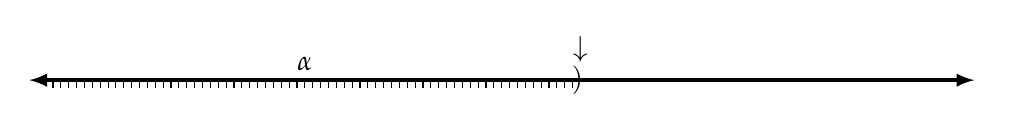
\begin{tikzpicture}
        \draw[latex-latex, very thick] (-6, 0) -- (6,0) node[anchor=south] {$\QQ$};
        \foreach \i in {-5.7,-5.6,...,0.9}{ 
        \draw[] (\i,0) -- (\i,-0.1);
        }
        \draw[] (1,0.1) node[anchor=south] {$\downarrow$};
        \draw[] (0.96,0) node[] {$)$};
        \draw[] (-2.5, 0) node[anchor=south] {$\alpha$};
    \end{tikzpicture}
    \caption{Visualization of a cut $\alpha$. The real number being described of this cut can be thought of as the number at the right boundary (the arrow).}
    \label{fig2} 
\end{figure}
\noindent In a sense, a cut gives us a way of discussing the real numbers (in the way we are familiar with them already) without referring to them directly; much like we could formally define/refer to rationals as equivalence classes of ordered pairs.  

\noindent As a note, we could very well define cuts to be bounded below rather than above, and the following construction would still work out.

\begin{nblank}{Step 2: $\RR$ is an ordered set}
    We define $\alpha < \beta$ to mean $\alpha \subsetneq \beta$. We show that this makes $\RR$ into an ordered set. First checking transitivity, we have that if $\alpha < \beta$ and $\beta < \gamma$ then $\alpha < \gamma$ by the fact that set inclusion is transitive. Furthermore, at most one of $\alpha < \beta$, $\alpha = \beta$, and $\beta < \alpha$ hold; to see this is the case, suppose the first two fail. Then, $\alpha \nsubseteq \beta$. Hence, $\exists p \in \alpha$ with $p \notin \beta$. If $q \in \beta$, $q < p$  and hence $q \in \alpha$ by (II), so $\beta \subset \alpha$, and since $\beta \neq \alpha$ it follows that $\beta \subsetneq \alpha$. 
\end{nblank}

\begin{nblank}{Step 3: $\RR$ has the LUB property}
    We show that $\RR$ has the LUB property. To see this is the case, let $A \subset \RR$ with $A \neq \emptyset$, and suppose that there exists $\beta \in \RR$ that is an upper bound for $A$. We will now define $\gamma = \bigcup_{\alpha \in A}\alpha$ and prove that $\gamma \in \RR$ and $\gamma = \sup A$ (hence $A$ has a supremum and $\RR$ has the LUB property).

    Since $A \neq \emptyset$, $\exists \alpha_0 \in A$, and since $\alpha_0 \neq \emptyset$ (as it is a cut) and $\alpha \subset \gamma$, it follows that $\gamma \neq \emptyset$. Next, we have that $\gamma \subset \beta$, since $\alpha \subset \beta$ for every $\alpha \in A$, and hence $\gamma \neq \QQ$, that is, $\gamma \subsetneq \QQ$. Hence $\gamma$ satisfies property (I) of a cut. 

    Take $p \in \gamma$. Then $p \in \alpha_1$ for some $\alpha_1 \in A$. If $q < p$, then $q \in \alpha$ (as $\alpha$ is a cut) so $q \in \gamma$, satisfying property (II).

    Next, choose $r \in \alpha_1$ such that $r > p$, then $r \in \gamma$ (as $\alpha_1 \subset \gamma$) and hence $\gamma$ satisfies property (III). Hence $\gamma$ is a cut, and $\gamma \in \RR$.

    Finally, we show that $\gamma = \sup A$. Clearly, $\alpha \leq \gamma$ for all $\alpha \in A$, as $\gamma = \bigcup_{\alpha \in A}\alpha$, so $\gamma$ is an upper boun dof $A$. To show that it is the least upper bound, let $\delta < \gamma$ be a cut. Then, $\exists s \in \gamma$ such that $s \notin \delta$. Therefore, $\exists \alpha_2 \in A$ such that $s \in \alpha_2$; hence $\delta < \alpha_2$, so $\delta$ is not an upper bound for $A$, giving the desired result. 
\end{nblank}

\begin{nblank}{Step 4: Addition on $\RR$}
    \begin{ndef}{Addition}
        If $\alpha, \beta \in \RR$, we define $\alpha + \beta = \set{s + t: s \in \alpha, t \in \beta}$. Showing that this is a cut is left as an exercise.
    \end{ndef}
    \begin{ndef}{Zero}
        $0^* = \set{s \in \QQ}$. Showing that this is a cut is left as an exercise.
    \end{ndef}

    We leave it as an exercise to show that the addition axioms (A1)-(A5) of a field are satisfied under this definition of addition on $\RR$, with the 0 element as $0^*$ defined above.
\end{nblank}

\begin{nblank}{Step 5: $\RR$ satisfies the Ordered Field Property (i)}
    We verify that if $\alpha, \beta, \gamma \in \RR$ and $\beta < \gamma$, then $\alpha + \beta < \alpha + \gamma$. 

    For every $s \in \alpha, t \in \beta$, we have that $t \in \gamma$ as $\beta$ is a subset of $\gamma$ by the definition of order on $\RR$. Hence, $s + t \in \alpha + \beta$ implies $s + t \in \alpha + \gamma$. Therefore, $\alpha + \beta \subseteq \alpha + \gamma$ and hence $\alpha + \beta \leq \alpha + \gamma$. 

    We are then left to check that $\alpha + \beta \neq \alpha + \gamma$. To see that this is the case, if $\alpha + \beta = \alpha + \gamma$, then $\beta = \alpha + \beta - \alpha = \alpha + \gamma - \alpha = \gamma$ by the field axioms for addition. Therefore we obtain that $\beta = \gamma$, contradicting that $\beta < \gamma$. Hence the claim is proven.

    As a remark, note that $0^* < \alpha \iff -\alpha < 0^*$.
\end{nblank}
\noindent Next we will define multiplication on $\RR$. A first attempt would be $\alpha \cdot \beta = \set{s \cdot t: s\in \alpha, t \in \beta}$. However, this definition is incosistent with negative numbers from what we require multiplication to accomplish. $-1 \cdot -1$ would fail to be a cut (it would not contain any negative numbers and hence fail criteria (II)) and $-1 \cdot 1$ would yield the entirety of the rationals (again not a cut!)

\begin{nblank}{Step 6: Positive Multiplication on $\RR$}
    \begin{ndef}{Positive Reals}
        We define $\RR^+ = \set{\alpha \in \RR: \alpha > 0^*}$
    \end{ndef}
    \begin{ndef}{Multiplication of Positive Reals}
        If $\alpha, \beta \in \RR^+$, we define $\alpha \cdot \beta = \set{r \cdot s: r \in \alpha, r> 0, s \in \beta, s > 0} \cup \set{t \in \QQ, t \leq 0}$. Equivalently, $\alpha \cdot \beta = \set{p \in \QQ:  \leq r \cdot s: r \in \alpha, r > 0, s \in \beta, s > 0}$. We leave it as an exercise to show that $\alpha \cdot \beta \in \RR$, and moreover, $\alpha \cdot \beta \in \RR^+$. Showing this second fact proves ordered field property (ii).
    \end{ndef}
    \begin{ndef}{One}
        $1^* = \set{r \in \QQ: r < 1}$. We again leave showing $1^* \in \RR^+$ as an exercise. 
    \end{ndef}
\end{nblank}

\begin{nblank}{Step 7: Multiplication on all of $\RR$}
    \begin{ndef}{Multiplication by zero}
        $\alpha \cdot 0^* = 0^* = 0^* \cdot \alpha$
    \end{ndef}
    \begin{ndef}{Multiplication}
        We define general multiplication as below, where the $\cdot$ on the RHS represents the multiplication of positive reals as outlined in Step 5. 
        \begin{align*}
            \alpha \cdot \beta = 
            \begin{cases}
            (-\alpha)\cdot(-\beta) & \text{if $\alpha < 0^*$ and $\beta < 0^*$}
            \\ -\left((-\alpha)\cdot\beta\right) & \text{if $\alpha < 0^*$ and $\beta > 0^*$}
            \\ -\left(\alpha \cdot (-\beta)\right) & \text{if $\alpha > 0^*$ and $\beta < 0^*$}
            \end{cases}
        \end{align*}
    \end{ndef}
    We leave it as an exercise to show that the multiplicative axioms (M1)-(M5), as well as the distributive law (D) of a field are satisfied under this definition of multiplication on $\RR$. 
\end{nblank}
\noindent Up until this point, we have shown $\RR$ is an ordered field with the LUB property; we last check that it contains $\QQ$ as a subfield. Note that we do have to be a bit careful with what we mean here; $\RR$ does not literally contain $\QQ$; $\RR$ is indeed a set of proper subsets of $\QQ$. What we really mean is to associate every element of $\QQ$ to an element of $\RR$ such that the field structure is preserved. 
\begin{nblank}{Step 8: $\RR$ contains $\QQ$ as a subfield}
    For each $r \in \QQ$, associate the cut $r^* = \set{p \in \QQ, p < r^*}$. We then leave as an easy exercise to verify that $r^* < s^* \iff r < s$, $r^* + s^* = r + s$, and $r^*\cdot s^* = r\cdot s$. This concludes the construction of the reals. \qed
\end{nblank}
\noindent Note that later on in the course, we will construct the real numbers in a different fashion; by considering Cauchy sequences modulo an equivalence relation. Also note that from here on out, it will suffice to have the standard/traditional picture of a "real number" in mind (i.e. infinite decimal expansions) and we will not have to really think about the real numbers as cuts; this was just necessary for the formal construction.

\subsection{The Complex Field}
\setcounter{rudin}{23}
\begin{definition}{The Complex Numbers}{1.24}
    We define the set of complex numbers to be $\CC = \set{(a, b): a, b \in \RR}$. For $x = (a, b) \in \CC$ and $y = (c, d) \in \CC$, we write $x = y$ if and only if $a = c$ and $b = d$ (note that this is a very different notion of equality compared to the rationals). We define the zero element to be $(0, 0)$ and the one element to be $(1, 0)$. We define addition of complex numbers such that:
    \begin{align*}
        x + y = (a, b) + (c, d) = (a + c, b + d)
    \end{align*}
    And multiplication of complex numbers such that:
    \begin{align*}
        x\cdot y = (a, b)\cdot (c, d) = (ac - ba, ad + bc)
    \end{align*}
\end{definition}
\begin{theorem}{$\CC$ is a field}{1.25}
    The operations of $+$ and $\cdot$, as well as the zero/one elements defined above turn $\CC$ into a field. 
\end{theorem}
\begin{nproof}
    It suffices to verify the field axioms (A1)-(A5), (M1)-(M5), and (D). We will here show (M3), (M4), and (M5) and leave the rest as exercises. 
    \begin{enumerate}[start=3, label={(M\arabic*):}]
    \item Let $x, y, z \in \CC$. We show that $(x\cdot y)\cdot z = x \cdot (y \cdot z)$. 
    \end{enumerate}
    
\end{nproof}
\subsection{The Cauchy-Shwartz Inequality}

\subsection{Euclidean Space}



\section{Basic Topology}
\subsection{Finite and Countable Sets}
This chapter is split into two portions; the first looks at counting, what it means for us to say that two sets have the same number of elements, and concludes with a classic theorem of Cantor concerning uncountable sets. The second part looks at abstract topological properties of sets, before moving onto the topology of the real numbers. 

Let us then begin with our discussion of counting. 
\newpage
\section{Numerical Sequences and Series}
\subsection{Sequences}
We begin by formally defining a sequence.
\begin{ndef}{: Sequences}{}
    Let $X$ be a metric space. A \textbf{sequence} is a function $f: \NN \mapsto X$. We can denote a term in the sequence as $f(n) = x_n$, or the entire sequence as $\set{x_n}_{n=1}^\infty$, $\set{x_n}$, $(x_n)$, or $\set{x_1, x_2, x_3 \ldots}$. 
\end{ndef}
\noindent We now discuss the notion of convergence of a sequence. Intuitively, we can equate convergence with the notion of points getting closer together.
\begin{definition}{Convergence of Sequences}{3.1}
    A sequence $\set{p_n}_{n=1}^\infty$ \textbf{converges} to $p \in X$ if for all $\e > 0$, there exists $N \in \NN$ such that $n \geq N$ implies $d(p_n, p) < \e$. In this case, we say that $\set{p_n}$ converges to $p$, or that $p$ is the limit of $\set{p_n}$, and denote this as $p_n \rightarrow p$ or $\lim_{n \rightarrow \infty} p_n = p$. If $\set{p_n}$ does not converge, we say it \textbf{diverges}.
\end{definition}
\noindent To phrase this definition in another way, we fix some $\e > 0$, and then we have that all points in the sequence past some $N \in \NN$ are contained in the neighbourhood $N_\e(p)$. In practice, it can be difficult to apply this definition of convergence if we don't know what the limiting $p$ is, as the definition implicitly uses the value of the limit. We will later discuss another definition of convergence (in $\RR^k$) that does not use the value of the limit.
\begin{figure}[htbp]
    \centering
    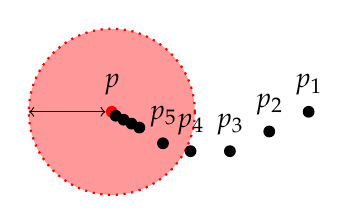
\begin{tikzpicture}[mycirc/.style={circle,fill, minimum size=0.15cm, inner sep = 0pt}]
        \draw[red, dotted, thick, fill = white!60!red] (-1, 0) circle (30pt);
        \node[mycirc, label=above:{$p$}, fill = red] at (-1, 0) {};
        \node[mycirc, label=above:{$p_1$}] at (1.5, 0) {};
        \node[mycirc, label=above:{$p_2$}] at (1, -0.25) {};
        \node[mycirc, label=above:{$p_3$}] at (0.5, -0.5) {};
        \node[mycirc, label=above:{$p_4$}] at (0, -0.5) {};
        \node[mycirc, label=above:{$p_5$}] at (-0.35, -0.4) {};
        \node[mycirc] at (-0.65, -0.2) {};
        \node[mycirc] at (-0.75, -0.15) {};
        \node[mycirc] at (-0.85, -0.1) {};
        \node[mycirc] at (-0.95, -0.05) {};
        \draw[<->] (-1.08, 0) -- (-2.05, 0);
        \node[label=above:{$\e$}] at (-1.5, -0.15) {};
    \end{tikzpicture}
    \caption{Visualization of a sequence $\set{p_n} \subset \RR^2$ converging to a point $p$. For the $\e > 0$ shown in the picture, we have that all points of the sequence past $N = 5$ lie in the open disk of radius $\e$ around $p$.}
    \label{fig15}
\end{figure}

\noindent As a remark, consider that convergence can depend on our choice of metric space; for example, $\set{\frac{1}{n}}$ as a sequence in $\RR$ converges to $0$, but the same sequence in the strictly positive reals ($\RR^+ = \set{x \in \RR: x > 0}$) does not converge.

Another interesting example (that again shows us the importance of the choice of metric space). Is $\RR$ equipped with the discrete metric. A question we can ask is ``given some points $p \in \RR$, what sequences converge to $p$?'' The answer turns out to be eventually constant sequences only; that is, sequences for which $p_n = p$ for $n \geq N$ for some $N$. 
\begin{proof}
    If $p_n \rightarrow p$, then setting $\e = \frac{1}{2}$, we have that there exists $N \in NN$ such that for all $n \geq N$, $d(p_n, p) < \e = \frac{1}{2}$. Under the discrete metric, this is only possible if $p_n = p$. 
\end{proof}
This of course is a strikingly different picture for $\RR$ with the standard metric of $d(x, y) = \abs{x - y}$. For example, the sequnce $p_n = \frac{1}{n}$ has no term equal to zero, but converges to $p = 0$. The takeaway message here can be that in the Euclidean metric, points can ``get closer'' but in the discrete metric, they cannot.

\stepcounter{rudin}
\begin{theorem}{}{3.3}
    Suppose $\set{s_n}, \set{t_n}$ are complex sequences that converge, with $\linf s_n \rightarrow s$ and $\linf t_n \rightarrow t$. Then:
    \begin{enumerate}
        \item $\linf(s_n + t_n) = s + t$.
        \item $\linf cs_n = cs$ and $\linf (c + s_n) = c + s$ for all $c \in \CC$.
        \item $\linf s_nt_n = st$
        \item $\linf \frac{1}{s_n} = \frac{1}{s}$ provided $s \neq 0$ and $s_n \neq 0$ for all $n$.
    \end{enumerate}
\end{theorem}
\begin{nproof}
    \begin{enumerate}
        \item Let $\e > 0$. There exist $N_1, N_2 \in \NN$ such that $\abs{s_{n_1} - s} < \frac{\e}{2}$ for $n_1 \geq N_1$ and $\abs{t_{n_2} - t} < \frac{\e}{2}$ for $n_2 \geq N_2$. Take $N = \max{N_1, N_2}$, and using the triangle inequality, it follows that for $n \geq N$:
        \begin{align*}
            \abs{(s_n + t_n) - (s + t)} \leq \abs{s_n - s} + \abs{t_n - t} < \frac{\e}{2} + \frac{\e}{2} = \e
        \end{align*} 
        We conclude that $\linf (s_n + t_n) = s + t$. 
        \item Let $\e > 0$. If $c = 0$ then the first sequence trivially converges to $0$, so suppose that $c \neq 0$. There exists $N$ such that $\abs{s_n - s} < \frac{\e}{\abs{c}}$ for $n \geq N$, so it follows that:
        \begin{align*}
            \abs{cs_n - cs} = \abs{c}\abs{s_n - s} < \abs{c}\frac{\e}{\abs{c}} = \e.
        \end{align*} For the second identity, we have that $c_n \rightarrow c$ for any constant sequence $c_n = c$ so we may apply (a).
        \item Let $\e > 0$. There exist $N_1, N_2$ such that $\abs{s_{n_1} - s} < \sqrt{2}$ for $n_1 \geq N_1$ and $\abs{t_{n_2} - t} < \sqrt{2}$ for $n_2 \geq N_2$. We then consider that:
        \begin{align*}
        s_nt_n - st = (s_n - s)(t_n - t) + s(t_n - t) + t(s_n - s)
        \end{align*}
        For $n \geq N = \max{N_1, N_2}$, we have that:
        \begin{align*}
            (s_n - s)(t_n - t) < \e
        \end{align*}
        And we hence observe that $\linf (s_n - s)(t_n - t) = 0$. We can then use (a) and (b) to find that:
        \begin{align*}
            \linf s(t_n - t) = 0, \quad \linf t(s_n - s) = 0
        \end{align*}
        So we conclude that $\linf (s_nt_n - st) = 0$ and hence $s_nt_n \rightarrow st$.
    \end{enumerate}
\end{nproof}
\begin{nproofcont}
    \begin{enumerate}
        \setcounter{enumi}{3}
        \item Choose $m$ such that $\abs{s_n - s} < \frac{1}{2}\abs{s}$ if $n \geq m$. We then have that $\abs{s_n} > \frac{1}{2}\abs{s}$ for $n \geq m$. Let $\e > )0$. Then, there exists $N$ with $N > m$ such that for $n \geq N$:
        \begin{align*}
            \abs{s_n - s} < \frac{1}{2}\abs{s}^2\e
        \end{align*}
        Hence, for $n \geq N$:
        \begin{align*}
            \abs{\frac{1}{s_n} - \frac{1}{s}} = \abs{\frac{s_n - s}{s_ns}} < \frac{2}{\abs{s}^2}\abs{s_n - s} < \e
        \end{align*}
        \qed
    \end{enumerate}
\end{nproofcont}

\begin{nlemma}{: Squeeze Lemma}{}
    Let $\set{x_n}$, $\set{s_n}$ be real-valued sequences. Then, if $0 \leq x_n \leq s_n$ for all $n$, and $\linf s_n = 0$, then $\linf x_n = 0$.
\end{nlemma}
\begin{nproof}
    Let $\e > 0$. Choose $N \in \NN$ such that $n \geq N$ implies $0 \leq s_n < \e$. Then, we have that for $n \geq N$, $0 \leq x_n \leq s_n < \e$ and hence $x_n \rightarrow 0$ as claimed. \qed
\end{nproof}

\noindent Note that we can prove a more generalized version of the Squeeze Lemma. Suppose we have sequences $\set{l_n}, \set{x_n}, \set{u_n}$ such that $l_n \leq x_n \leq u_n$ for all $n$ and $\linf l_n = \linf u_n = L \in \RR$. Then, $\linf x_n = L$.
\begin{proof}
    We have that $0 \leq a_n - l_n \leq u_n - l_n$. We have that $\linf u_n - l_n = 0$ by Theorem \ref{thm:3.3}(a), so by the (original) Squeeze Lemma we have that $\linf a_n - l_n = 0$. It then follows that $\linf a_n = \linf l_n = L$ as claimed.
\end{proof}

\setcounter{rudin}{19}
\begin{theorem}{}{3.20}
    \begin{enumerate}
        \item Let $p > 0$. Then, $\linf \frac{1}{n^p} = 0$.
        \item Let $p > 0$. Then, $\linf \sqrt[n]{p} = 1$.
        \item $\linf \sqrt[n]{n} = 1$.
        \item Let $p > 0$ and $\alpha \in \RR$. Then, $\linf \frac{n^\alpha}{(1+p)^n} = 0$.
        \item Let $\abs{x} < 1$. Then, $\linf x^n = 0$. 
    \end{enumerate}
\end{theorem}
\begin{nproof}
    \begin{enumerate}
        \item Let $\e > 0$. Choose $N$ such that $\frac{1}{N^p} < \e$, namely $N > \left(\frac{1}{\e}\right)^{1/p}$. Then, for $n \geq N$, $\frac{1}{n^p} < \frac{1}{N^p} < \e$. 
        
        \item If $p = 1$, the sequence is constant and the conclusion immediate. 
        
        If $p > 1$, then let $x_n = \sqrt[n]{p} - 1$. We then have that:
        \begin{align*}
            p = (x_n + 1)^n = \sum_{k=0}^n \binom{n}{k}x_n^k \geq nx_n
        \end{align*}
        Where the second equality follows from the binomial theorem (where $\binom{n}{k} = \frac{n!}{k!(n-k)!}$), and the inequality follows by considering that we just keep the $k = 1$ term (and the series is non-negative). Hence, we have that $x_n \leq \frac{p}{n}$, and $x_n \rightarrow 0$ by (a). 
        
        If $p < 1$, then let $q = \frac{1}{p} > 1$. Then, $\sqrt[n]{q} \rightarrow 1$ by the argument above. By Theorem \ref{thm:3.3}(d), we then have that $\sqrt[n]{p} = \frac{1}{\sqrt[n]{q}} \rightarrow \frac{1}{1} = 1$.

        \item Let $x_n = \sqrt[n]{n} - 1$. Then, we have that:
        \begin{align*}
            n = (x_n + 1)^n = \sum_{k=0}^n\binom{n}{k}x_n^k \geq \frac{n(n-1)}{2}x_n^2
        \end{align*}
        Where the inequality follows from keeping the $k = 2$ term only. We then have that $x_n \leq \sqrt{\frac{2}{n-1}}$ and hence $x_n \rightarrow 0$ by the Squeeze Lemma.
        \item We want to show $\frac{n^\alpha}{(1+p)^n} \rightarrow 0$; we therefore want an upper bound on the expression, and hence a lower bound on $(1+p)^n$. Applying the Binomial Theorem we have that:
        \begin{align*}
            (1+p)^n = \sum_{k=0}^n\binom{n}{k}p^k = \left((n)(n-1)(n-2)\cdots(n-k+1)\right)\frac{p^k}{n!}
        \end{align*}
        Now, we pick $k > \alpha$. For $2n > k$, we then have that:
        \begin{align*}
            (1+p)^n \geq \left(\frac{n}{2}\right)^k\frac{p^k}{k!}
        \end{align*}
        We therefore have that:
        \begin{align*}
            \frac{n^\alpha}{(1+p)^k} \leq \frac{2^kk!}{p^k}n^{\alpha - k} \rightarrow 0
        \end{align*}
        And the claim follows by the Squeeze Lemma.
        
        \item Taking $\alpha = 0$ in (d), the claim follows by setting $\abs{x} = \frac{1}{1+p} < 1$ (as $p > 0$) and recognizing that $x_n \rightarrow 0 \iff \abs{x^n} = \abs{x}^n \rightarrow 0$. \qed
    \end{enumerate}
\end{nproof}

\subsection{Subsequences}

\setcounter{rudin}{1}
\begin{theorem}{}{3.2}
    Let $\set{p_n}$ be a sequence in $X$.
    \begin{enumerate}
        \item $p_n \rightarrow p$ in $X$ if and only if for all $r > 0$, $N_r(p)$ contains all but finitely many points of $\set{p_n}$.
        \item If $p_n \rightarrow p$ and $p_n \rightarrow p'$ then $p = p'$. In other words, the limit is unique.
        \item If $\set{p_n}$ is convergent, then it is bounded (that is, for any $q \in X$ there exists $M \in \RR$ such that $d(q, p_n) \leq M$ for all $n \in \NN$).
        \item If $E \subset X$ has a limit point $p$, then there exists $\set{p_n}$ in $E$ such that $p_n \rightarrow p$. 
    \end{enumerate}
\end{theorem}
\begin{nproof}
    \begin{enumerate}
        \item The claim follows immediately from the definition of convergence; for any $r = \e > 0$, there exists $N \in \NN$ such that $N_r(p)$ contains $\set{p_n: n \geq N}$.
        \item There exist $N_1, N_2$ such that $d(p, p_{n_1}) < \frac{\e}{2}$ if $n_1 \geq N_1$ and $d(p, p_{n_2}) < \frac{\e}{2}$ if $n_2 \geq N_2$. Then for $n \geq N = \max{N_1, N_2}$ we have (using the triangle inequality) that:
        \begin{align*}
            d(p, p') \leq d(p, p_n) + d(p_n, p') < \frac{\e}{2} + \frac{\e}{2} = \e
        \end{align*}
        Since $\e$ is arbitrary, $d(p, p') = 0$ and hence $p = p'$.

        \item If $p_n \rightarrow p$, there exists $N$ such that $d(p_n, p) < 1$ for all $n \geq N$. Set:
        \begin{align*}
            r = \max\set{1, d(p_1, p), d(p_2, p), \ldots ,d(p_{N-1}, p)}
        \end{align*}
        For any $q \in X$, we then have that:
        \begin{align*}
            d(q, p_n) \leq d(q, p) + d(p, p_n) \leq d(q, p) + r
        \end{align*}
        so the claim follows with $M = r + d(q, p) + 1$.
        \item Pick $p_n \in E$ such that $d(p_n, p) < \frac{1}{n}$. Let $\e > 0$, and $N > \frac{1}{\e}$. Then, $n \geq N$ implies $\frac{1}{n} \leq \frac{1}{N} < \e$ and hence $d(p_n, p) < \e$ for all $n \geq N$, and hence $p_n \rightarrow p$ as desired. \qed
    \end{enumerate}
\end{nproof}

\setcounter{rudin}{4}
\begin{definition}{Subsequences}{3.5}
    Given $\set{p_n}$ and $n_1 < n_2 < n_3 < \ldots$, we say that $\set{p_{n_j}}$ is a \textbf{subsequence} of $\set{p_n}$.
\end{definition}

\noindent We first consider some examples. Let $p_n = n$. Then some valid subsequences of $\set{p_n}$ are $\set{1, 2, 3, 4, 5, \ldots}$ (the original sequence), $\set{1, 3, 5, 7, \ldots}$ (the odds), $\set{2, 3, 5, 7, 11, 13, \ldots}$ (the primes). Next, let $p_n = i^n$. We have that $\set{p_n} = \set{i, -1, -i, 1, i, -1, -i, 1, \ldots}$ which is clearly divergent. However, the subsequences $\set{i, i, i, \ldots}$, $\set{-1, -1, -1, \ldots}$, $\set{-i, -i, -i, \ldots}$ and $\set{1, 1, 1, \ldots}$ are all convergent! It is hence possible for a divergent sequence to have a convergent subsequence.

\begin{nlemma}{}{}
    If $p_n \rightarrow p$, then every subsequence of $\set{p_n}$ converges to $p$. 
\end{nlemma}

\begin{nproof}
    Suppose $p_n \rightarrow p$ and let $\set{p_{n_j}}$ be a subsequence of $p_n$. Let $\e > 0$. Then, there exists some $N \in \NN$ such that $d(p, p_n) < \e$ if $n \geq N$. Hence, $d(p, p_{n_j}) < \e$ if $n_j \geq N$ and hence $p_{n_j} \rightarrow p$. \qed
\end{nproof}

\begin{theorem}{}{3.6}
    \begin{enumerate}
        \item If $\set{p_n} \subset X$ with $X$ compact, then $\set{p_n}$ has a convergenct subsequence.
        \item If $\set{p_n} \subset \RR^k$ and $\set{p_n}$ is bounded, then $\set{p_n}$ has a convergent subsequence.
    \end{enumerate}
\end{theorem}
\begin{nproof}
    \begin{enumerate}
        \item Let $E$ be the range of $\set{p_n}$. If $E$ is finite, then there exists $x \in X$ and $n_1 < n_2 < n_3 < \ldots$ such that $p_{n_j} = x$ for all $j$. Therefore $p_{n_j} \rightarrow x$ and we are done. If $E$ is infinite, then by compactness, $E \subset X$ has a limit point in $X$ by Theorem \ref{thm:2.37}. By Theorem \ref{thm:3.2}(d) there exists a sequence $\set{p_{n_j}}$ in $E$ such that $p_{n_j} \rightarrow p$.
        \item By Theorem \ref{thm:2.41}, $E$ (being bounded) lies in a compact subset of $\RR^k$. We then apply (a). \qed
    \end{enumerate}
\end{nproof}

\subsection{Cauchy Sequences and Completeness}

\setcounter{rudin}{7}
\begin{definition}{Cauchy Sequences}{3.8}
    A sequence $\set{p_n} \subset X$ is a \textbf{Cauchy sequence} if for all $\e > 0$, there exists $N \in \NN$ such that for all $n, m \geq N$, $d(p_n, p_m) < \e$. 
\end{definition}
\noindent Note the fact that this definition does not refer to a particular $p$ that the sequence may converge to! It instead formalizes the notion of the points of a sequence getting ``closer together'' as the sequence goes on. It is therefore easier to check if a sequence is Cauchy than if it converges, as we don't need to know the value of the limit. To this end, it is useful to know in what situations a sequence being Cauchy implies that the sequence is convergent. We will soon arrive at a theorem that addresses this question, but first we establish a little more machinery.

\begin{definition}{Diameter}{3.9}
    Let $E \subset X$. Then the \textbf{diameter} of $E$, denoted $\diam E$ is defined as $\diam E = \sup\set{d(p, q): p, q \in E}$. It follows from the definition that a sequence $\set{p_n}$ is Cauchy if and only if $\lim_{N \rightarrow \infty} \diam E_n = 0$ where $E_n = \set{p_n}_{n=N}^\infty$ (the tail of the sequence).
\end{definition}

\begin{nexample}{}{}
    \begin{enumerate}
        \item If $E = (a, b) \subset \RR$ or $E = [a, b] \subset \RR$, then $\diam E = b - a$.
        \item If $E = (0, 1) \times (0,1) \subset \RR^2$, then $\diam E = \sqrt{2}$ (the diagonal of the open square).
    \end{enumerate}
\end{nexample}

\begin{theorem}{}{3.10}
    \begin{enumerate}
        \item Let $E \subset X$. Then, $\diam \overline{E} = \diam E$.
        \item If $K_n \subset X$ are compact, $K_{n+1} \subset K_n$ for all $n$, and $\linf \diam K_n  = 0$, then $\bigcap_{n=1}^\infty K_n$ consists of exactly one point.
    \end{enumerate}
\end{theorem}

\begin{nproof}
    \begin{enumerate}
        \item Since $E \subset \overline{E}$, it is clear that $\diam \overline{E} \geq \diam E$. Next, let $\e > 0$ and $p, q \in \overline{E}$. Choose $p', q' \in E$ such that $d(p, p') < \frac{\e}{2}$, $d(q, q') < \frac{\e}{2}$ (this choice is possible as either $p, q$ are in $E$, or $p, q$ are limit points of $E$). Then, we have that:
        \begin{align*}
            d(p, q) \leq d(p, p') + d(p', q) \leq d(p, p') + d(p', q') + d(q', q) < \frac{\e}{2} + \diam E + \frac{\e}{2} = \diam E + \e
        \end{align*}
        $\e, p$, and $q$ are arbitrary, so it follows that $\diam \overline{E} \leq \diam E + \e$ from the definition of the diameter. It then follows that $\diam \overline{E} \leq \diam E$. We conclude that $\diam \overline{E} = \diam E$.
        \item Let $K = \bigcap_{n=1}^\infty K_n$. By the corollary to Theorem \ref{thm:2.36}, we have that $K \neq \emptyset$, so $K$ contains at least one point. Since $K \subset K_n$, it follows that $\diam K \leq \diam K_n$ for any $n$, and since $\diam K_n \rightarrow 0$, $\diam K = 0$. If there were $p, q \in K$ such that $p \neq q$, then $\diam K \neq 0$, so it must follow that $K$ has at most one point. We conclude that $K$ has exactly one point. \qed
    \end{enumerate}
\end{nproof}

\begin{nlemma}{}{}
    If a sequence $\set{p_n}$ is Cauchy, then it is bounded.
\end{nlemma}
\begin{nproof}
    If $\set{p_n}$ is Cauchy, then we have that $\lim_{N \rightarrow \infty} \diam E_N = \lim_{N \rightarrow \infty} \diam \set{p_n}_{n = N}^\infty = 0$. Then for some $N \in \NN$, $\diam E_N < 1$. The range of $\set{p_n}$ is the union of $E_N$ and the finite set $\set{p_1, \ldots, p_{N-1}}$ and hence $\set{p_n}$ is bounded. \qed
\end{nproof}

\begin{theorem}{}{3.11}
    \begin{enumerate}
        \item If a sequence $\set{p_n} \subset X$ converges, then it is Cauchy.
        \item If a sequence $\set{p_n} \subset X$ is Cauchy and $X$ is compact, then $\set{p_n}$ converges to some $p \in X$.
        \item In $\RR^k$, every Cauchy sequence is convergent.
    \end{enumerate}
\end{theorem}

\begin{nproof}
    \begin{enumerate}
        \item Let $p_n \rightarrow p$ and let $\e > 0$. There exists $N \in \NN$ such that $d(p_n, p) < \frac{\e}{2}$ if $n \geq N$. Then, for $n, m \geq N$, we have that:
        \begin{align*}
            d(p_n, p_m) \leq d(p_n, p) + d(p, p_m) < \frac{\e}{2} + \frac{\e}{2} = \e
        \end{align*}
        so $\set{p_n}$ is Cauchy.
        \item Let $E_N = \set{p_n}_{n = N}^{\infty}$. Then, $\overline{E}_N \subset X$ is closed, so by the compactness of $X$ we have that $\overline{E}_N$ is compact by Theorem \ref{thm:2.35}. Since $E_{N+1} \subset E_N$, we have that $\overline{E}_{N+1} \subset \overline{E}_N$, and additionally we have that $\lim_{N \rightarrow \infty} \overline{E}_N =\lim_{N \rightarrow \infty} E_N = 0$ where the first equality follows from Theorem \ref{thm:3.10}(a) and the second equality follows from the fact that $\set{p_n}$ is Cauchy and Definition \ref{def:3.9}. Thus, Theorem \ref{thm:3.10}(b) says that there exists a unique point $p \in \bigcap_{n=1}^\infty \overline{E}_N$. Next, let $\e > 0$. Then, there exists $N_0$ such that $\diam \overline{E}_N < \e$ for all $N \geq N_0$. So, $d(p, q) < \e$ for all $q \in \overline{E}_N$, so the same holds for all $q \in E_N$. Hence, $d(p, p_n) < \e$ for all $n \geq N_0$, which shows that $p_n \rightarrow p$ and proves the claim. 
        \item By the above Lemma, Cauchy sequences are bounded. Hence, $\set{p_n} \subset I$ for some $k$-cell $I \subset \RR^k$. Since $I$ is compact in $\RR^k$, the claim follows from (b). \qed
    \end{enumerate}
\end{nproof}

\begin{definition}{Completeness}{3.12}
    A metric space $X$ is called \textbf{complete} if every Cauchy sequence converges in $X$. 
\end{definition}
It might be tempting at first to think that every space would be complete, but this is not the case. For example, something that can go wrong is a sequnece can be Cauchy, but the limit can lie ``outside'' of the space. To see this, consider again the sequence $\set{\frac{1}{n}}$ in the metric space $\RR^+ = \RR \setminus \set{x \in \RR: x \leq 0}$. The sequence is Cauchy, but does not converge in $\RR^+$ (as it converges to 0, which lies outside of the space).

\begin{nexample}{}{}
    \begin{enumerate}[(i)]
        \item Compact sets are complete by Theorem \ref{thm:3.11}(b).
        \item $\RR^k$ (and $\CC$) are complete by Theorem \ref{thm:3.11}(c).
        \item $\QQ$ is not complete. We can make a sequence of rational points that converges to an irrational number in $\RR$ which is Cauchy, but does not converge in $\QQ$ (Example \ref{exam:1.1b} gives a way one might construct such a sequence). 
    \end{enumerate}
\end{nexample}
\noindent Note that $\QQ$ can be completed to $\RR$, and in general for any $(X, d)$ which is not complete, there exists $(X^*, d^*)$ that is complete such that $\abs{X} = X^*$. Indeed, this is another way we can construct the real numbers! $\RR$ can be viewed as equivalence classes of Cauchy sequences in $\QQ$. The idea is to define an equivalnence relation $\sim$ such that $p_n \sim q_n$ if $\linf d(p_n, q_n) = 0$. $X^*$ is then defined as the set of equivalence classes under that equivalence relation, equipped with the metric $d^*([p], [q]) = \linf d(p_n, q_n)$. It can then be checked that $d^*$ is a valid metric and that $X^*$ is complete. For the full proof, see HW7, or exercises 3.23-3.25 in Rudin (note: this proof is quite technical/difficult).

To motivate the next theorem, consider that all convergent sequences in $\RR$ (and in general) are bounded (as we saw in Theorem \ref{thm:3.2}(c)). However, this is not always true; for example consider $p_n = (-1)^n$ which is clearly bounded but divergent. What then are conditions that a bounded sequence may converge?

\begin{definition}{Monotonic Sequences}{3.13}
    A sequence $\set{p_n} \subset \RR$ is \textbf{monotonically increasing} if $p_{n+1} \geq p_n$ for all $n$, and \textbf{montonically decreasing} if $p_{n+1} \leq p_n$.
\end{definition}

\begin{theorem}{}{3.14}
    Suppose $\set{p_n} \subset \RR$ is montonic. Then, $\set{p_n}$ is convergent if and only if it is bounded. 
\end{theorem}

\begin{nproof}
    $\boxed{\implies}$ See Theorem \ref{thm:3.2}(c).

    $\boxed{\impliedby}$ We show the proof for the increasing case as the decreasing case is analogous. Let $p = \sup{p_n: n \in \NN}$ which exists as $\set{p_n}$ is bounded and $\RR$ has the LUB property. Then, $p_n \leq p$ for all $n$. Let $\e > 0$. Then, there exists $N \in \NN$ such that $p - \e < p_{N} < p_{N+1}$. By the monotonicity of $\set{p_n}$, it follows that $\abs{p_n - p} < \e$ for all $n \geq N$. Hence, $p_n \rightarrow p$. \qed
\end{nproof}

\begin{definition}{Limits to Infinity}{3.15}
    Let $\set{p_n} \subset \RR$. If for all $M \in \RR$, there exists $N \in \NN$ such that $p_n > M$ for all $n \geq N$, then we write $p_n \rightarrow \infty$. If instead for all $M \in \RR$ there exists $N \in \NN$ such that $p_n < M$ for all $n \geq N$, then we write $p_n \rightarrow -\infty$.
\end{definition}



\subsection{Limsup and Liminf}
\subsection{Series}
\subsection{The Harmonic Series and Euler's Number}
\subsection{Convergence Tests}
\subsection{Power Series}


\newpage 
\section[Continuity]{\hyperlink{toc}{Continuity}}

\subsection{Limits and Continuity}
\begin{definition}{Limits}{4.1}
    Let $X, Y$ be metric spaces. Let $E \subset X$, and let $f: E \mapsto Y$. Let $p \in X$ be a limit point of $E$. Then, we say that $\lim_{x\rightarrow p} f(x) = q$ or $f(x) \rightarrow q$ as $x \rightarrow p$ if there exists $q \in Y$ such that for all $\e > 0$, there exists $\delta > 0$ such that for all $x \in E$ with $0 < d_X(x, p) < \delta$ we have that $d_Y(f(x), q) < \e$. 
\end{definition}
\begin{figure}[htbp]
    \centering
    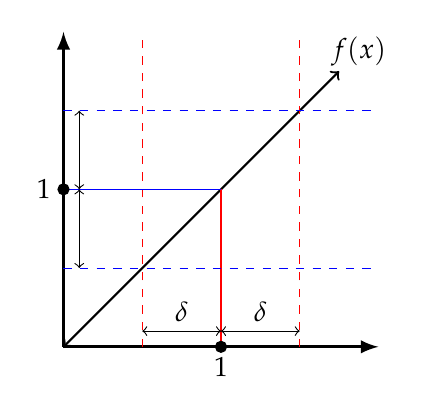
\begin{tikzpicture}[scale=2]
        \draw[-latex,very thick] (0,0)--(2,0);
        \draw[-latex,very thick] (0,0)--(0,2);
        \draw[<->, thick] (0, 0) -- (1.75, 1.75);
        \draw[color = red] (1, 0) -- (1, 1);
        \draw[color = red, dashed] (0.5, 0) -- (0.5, 2);
        \draw[color = red, dashed] (1.5, 0) -- (1.5, 2);
        \draw[<->] (0.5, 0.1) -- (1, 0.1);
        \node[above] at (0.75, 0.1) {$\delta$};
        \draw[<->] (1, 0.1) -- (1.5, 0.1);
        \node[above] at (1.25, 0.1) {$\delta$};
        \draw[color = blue] (0, 1) -- (1, 1);
        \draw[color = blue, dashed] (0, 0.5) -- (2, 0.5);
        \draw[color = blue, dashed] (0, 1.5) -- (2, 1.5);
        \draw[<->] (0.1, 0.5) -- (0.1, 1);
        \node[right] at (0.1, 0.75) {$\e$};
        \draw[<->] (0.1, 1) -- (0.1, 1.5);
        \node[right] at (0.1, 1.25) {$\e$};
        \draw[fill = black] (0, 1) circle (1pt);
        \node[xshift = -0.25cm] at (0, 1) {$1$};
        \draw[fill = black] (1, 0) circle (1pt);
        \node[yshift = -0.25cm] at (1, 0) {$1$};
        \node[yshift = 0.25cm, xshift = 0.25cm] at (1.75, 1.75) {$f(x)$};
    \end{tikzpicture}
    \caption{Visualization of the limit $\lim_{x \rightarrow 1}f(x) = 1$ for $f(x) = x$. For any $\e > 0$, we can take $\delta = \e$ and then we have that $\abs{f(x) - 1} < \e$ if $\abs{x - 1} < \delta$.}
    \label{fig17}
\end{figure}
Note in the above definition that we do not care about $f(p)$, that is, the actual value of $f$ at $p$. In particular, if $p \notin E$, then $f(p)$ is not even necessarily defined. This distinction between the limit and the actual value of a function at a point becomes crucial later on when we want to define a derivative. Although we will discuss this in more detail in Chapter 5, the definition of a derivative of a function $g$ at a point $p \in \RR$ involves the function $f: \RR \rightarrow \RR$ such that:
\begin{align*}
    f(x) = \frac{g(x) - g(p)}{x - p}
\end{align*}
Evidently, the domain of $f$ does not contain the point $p$, but we are interested in the value of $f$ in the limit of $x \rightarrow p$ (which, if it exists, is the value of the derivative).

\begin{figure}[htbp]
    \centering
    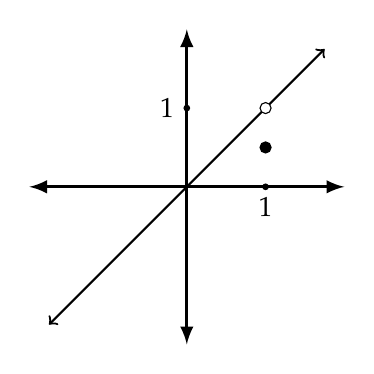
\begin{tikzpicture}
        \draw[latex-latex,very thick] (-2,0)--(2,0);
        \draw[latex-latex,very thick] (0,-2)--(0,2);
        \draw[<->, thick] (-1.75, -1.75) -- (1.75, 1.75);
        \draw[fill = black] (0, 1) circle (1pt);
        \node[xshift = -0.25cm] at (0, 1) {$1$};
        \draw[fill = black] (1, 0) circle (1pt);
        \node[yshift = -0.25cm] at (1, 0) {$1$};
        \draw[fill = white] (1, 1) circle (2pt);
        \draw[fill = black] (1, 0.5) circle (2pt);
    \end{tikzpicture}
    
    \caption{Visualization of the function $f(x) = x$ for $x \in \RR \setminus \set{1}$, $f(x) = 0$ for $x = 1$. In this case, we have that $f(1) = 0$ but $\lim_{x \rightarrow 1} f(x) = 1$, demonstrating that the actual value of the function is irrelevant when defining the limit.}
    \label{fig18}
\end{figure}

\begin{theorem}{}{4.2}
    Let $X, Y$ be metric spaces. Let $E \subset X$ and $f:E \mapsto Y$. Suppose that for all sequences $\set{p_n} \subset E$ with $p_n \rightarrow p$ and $p_n \neq p$, we have that $f(p_n) \rightarrow q \in Y$. Then, this is equivalent to saying that $\lim_{x \rightarrow p} f(x) = q$.
\end{theorem}
\begin{nproof}
    \boxed{\implies} Suppose that $\lim_{x \rightarrow p} f(x) = q$, and let $\set{p_n}$ be a sequence in $E$ with $p_n \rightarrow p$ and $p_n \neq p$ for all $n$. We wish to show that $f(p_n) \rightarrow q$. Let $\e > 0$. We show that there exists $N \in \NN$ such that $d_Y(f(p_n), q) < \e$ for all $n \geq N$. Since $\lim_{x \rightarrow p} f(x) = q$, there exists $\delta > 0$ such that for all $x \in E$ with $d_X(p, x) < \delta$, $d_Y(f(x),q) < \e$. Since we know that $p_n \rightarrow p$, there exists some $N$ such that $0 < d(p_n, p) < \delta$ for all $n \geq N$, so we have that $d_Y(f(p_n), q) < \e$ as required. 

    \boxed{\impliedby} We show the contrapositive. Suppose that $\lim_{x \rightarrow p} f(x) \neq q$. We wish to find a sequence $\set{p_n} \subset E$ with $p_n \rightarrow p$ and $p_n \neq p$ for all $n$ such that $f(p_n)$ does not converge to $q$. Since $\lim_{x \rightarrow p} f(x) \neq q$, then there exists $\e > 0$ such that for all $\delta > 0$, there exists $x \in E$ such that $0 < d_X(x, p) < \delta$ but $d_Y(f(x), q) \geq \e$. For each $\delta$ of the form $\frac{1}{n}$, let $p_n \in E$ be the corresponding value of $x$. Then, $p_n \rightarrow p$, $p_n \neq p$ for all $n$, and $f(p_n)$ does not converge to $q$ as $d(f(p_n), q) \geq \e$ for all $n$. \qed
\end{nproof}

\stepcounter{rudin}

\begin{theorem}{}{4.4}
    When $Y = \CC$ (i.e. the functions we consider are complex), then limits respect sums, differences, products, and functions. That is, let $X$ is a metric space, $E \subset X$, and $f, g: E \mapsto \CC$ with $p$ a limit point of $E$. If $\lim_{x \rightarrow p}f(x) = q$ and $\lim_{x \rightarrow p}g(x) = r$, then $\lim_{x \rightarrow p}(f+g)(x) = q + r$. The same holds for subtraction, multiplication, and division (provided we do not divide by zero).
\end{theorem}
\begin{nproof}
    By Theorem \ref{thm:4.2}, these properties of limits follow from the analogous properties of sequences (Theorem \ref{thm:3.3}).
\end{nproof}

\begin{definition}{Continuity}{4.5}
    Let $X, Y$ be metric spaces, and $E \subset X$. Let $p \in E$, and define $f: E \mapsto Y$. We say that $f$ is \textbf{continuous} at $p$ if for all $\e > 0$, there exists $\delta > 0$ such that for all $x \in E$ with $d_X(x, p) < \delta$, we have that $d_Y(f(x), f(p)) < \e$. Equivalently, $f(N_\delta^E(p)) \subset N_\e^Y(f(p))$. If $f$ is continuous at $p$ for all $p \in E$, we say that $f$ is continuous.
\end{definition}
\noindent Note that this definition of continuity is heavily reliant on the particular metric of $X$ and $Y$; in particular, there can be functions that are continuous for some choices of metric but not others.

Let us consider some examples of continuous functions (while thinking about different possible metric spaces). 

First, let us take onsider $X = E = \ZZ$ and $Y = \RR$. What functions $f: E \rightarrow Y$ are continuous at $p = 0$? The answer turns out to be all functions! To see this, fix $n \in \ZZ$ and let $\e > 0$. We then have that if $\abs{n - m} < \frac{1}{2}$, then $\abs{f(n) - f(m)} < \e$ as the only point $m$ contained in $N_{1/2}^\ZZ(n)$ is $n$ itself (and hence $\abs{f(n) - f(m)} = \abs{f(n) - f(n)} = 0$). This argument applies to every $n \in \ZZ$ and hence all functions $f: \ZZ \mapsto \RR$ are continuous.

As further examples (that work for arbitrary metric spaces), If we have that $f: X \mapsto X$, $f(x) = x$, we have that $f$ is continuous (pick $\delta = \e$ in the definition of continuity). If we have that $f: X \mapsto Y$, $f(x) = c$ for some $c \in Y$, then $f$ is also continuous (pick any $\delta > 0$ in the definition). 

Finally, the above definition doesn't make a distinction between limit points and isolated points. However, it turns out that according to the definition, if $p \in E$ is isolated, then every function $f$ with $E$ as its domain is continuous. To see this, consider that for any $\e > 0$, we can pick $\delta > 0$ such that the only point $x \in E$ for which $d_X(x, p) < \delta$ is $x = p$ (such a choice of $\delta$ is possible as $p$ is isolated). It then follows that $d_Y(f(x), f(p)) = 0 < \e$. 
 
We now consider a Theorem which gives us a familiar notion of continuity (that may have been encountered in first year calculus).

\begin{theorem}{}{4.6}
    Suppose that $p$ is a limit point of $E$ in Definition \ref{def:4.5}. Then, $f$ is continuous at $p$ if and only if $\lim_{x \rightarrow p}f(x) = f(p)$. 
\end{theorem}
\begin{nproof}
    The claim immediately follows by comparing Definitions \ref{def:4.1} and \ref{def:4.5}. \qed
\end{nproof}

\begin{theorem}{}{4.7}
    Let $X, Y, Z$ be metric spaces, and $E \subset X, F \subset Y$. Let $f: E \mapsto Y$, $g: F \mapsto Z$, and suppose $f(E) \subset F$. Let $p \in E$. If $f$ is continuous at $p$ and $g$ is continous at $f(p)$, then $g \circ f: E \mapsto Z$ is continuous at $p$.
\end{theorem}
\begin{nproof}
    Let $\e > 0$. Since $g$ is continuous at $f(p)$, there exists $\gamma > 0$ such that $d_Z(g(y), g(f(p))) < \e$ if $d_Y(y, f(p)) ,< \gamma$. Since $f$ is continuous at $p$, there exists $\delta > 0$ such that $d_Y(f(x), f(p)) < \gamma$ if $d_X(x, p) < \delta$. Hence, we have that $d_Z(h(x), h(p)) = d_Z(g(f(x)), g(f(p))) < \e$ if $d_X(x, p) < \delta$ and $x \in E$. We conclude that $h$ is continuous at $p$. \qed
\end{nproof}

\subsection{Topological Characterization of Continuity}
\begin{theorem}{}{4.8}
    Let $X, Y$ be metric spaces, and $f: X \mapsto Y$. Then, $f$ is continuous if and only if $f^{-1}(V) \subset X$ is open for every open set $V \subset Y$.
\end{theorem}
\begin{nproof}
    \boxed{\implies} Suppose $f$ is continuous, and $V \subset Y$ is open. Let $p \in f^{-1}(V)$, so $f(p) \in V$. $V$ is open, so it follows that $f(p)$ is an interior point of $V$. So, there exists $r > 0$ such that $N_r^Y(f(p)) \subset V$. Next, $f$ is continuous, so there exists $\delta > 0$ such that for all $x \in X$ with $d_X(x, p) < \delta$, $d_Y(f(x), f(p)) < r$. Hence, we obtain that $f(x) \in N_r^Y(f(p)) \subset V$. In particular, $N_\delta^X(p) \subset f^{-1}(V)$, so $p$ is an interior point of $f^{-1}(V)$. Hence every point of $f^{-1}(V)$ is an interior point, and $f^{-1}(V)$ is open.

    \boxed{\impliedby} Suppose $f^{-1}(V)$ is open for every open set $V \subset Y$. Let $p \in X$ and $\e > 0$. Let $V = N_\e^Y(f(p))$ which is open, so by assumption $f^{-1}(V)$ is open. $p \in f^{-1}(V)$, so $p$ is an interior point. Hence, there exists $\delta > 0$ such that $N_\delta^X(p) \subset f^{-1}(V)$. In other words, if $d_X(x, p) < \delta$, then $f(x) \in V$, so $d_Y(f(x), f(p)) < \e$. $f$ is then continuous by definition. \qed
\end{nproof}

\begin{ncorollary}{}{}
    $f: X \mapsto Y$ is continuous if and only if $f^{-1}(F) \subset X$ is closed for every closed set $F \subset Y$.
\end{ncorollary}
\begin{nproof}
    Let $V = F^c$ with $V$ open. Then, the above statement is equivalent to saying that a function $f: X \mapsto Y$ is continuous if and only if $f^{-1}(V^c) = \left(f^{-1}(V)\right)^c$ is closed for every open set $V \subset Y$. This is equivalent to the statement that $f^{-1}(V)$ is open for every open set $V \subset Y$, and the claim follows by the previous theorem. \qed
\end{nproof}

\noindent Note that the above topological characterization says properties of sets are preserved under taking the preimage; it does not say anything about preserving properties under the image. That is to say, images of open/closed sets are not necessarily open/closed.

\begin{nexample}{}{}
    Consider $X = \RR^+ = (0, \infty)$ and $Y = \RR$. Then, the function:
    \begin{align*}
        \fullfunction{f}{X}{Y}{x}{\frac{1}{x}}
    \end{align*}
    is continuous. Then defining $A = [1, \infty)$ we have that $A$ is closed, but $f(A) = (0, 1]$ is not closed.   
\end{nexample}


\begin{theorem}{}{4.9}
    Let $f: X \mapsto \CC$ and $g: X \mapsto \CC$ be continous functions. Then, $f+g$, $fg$ are continuous, and $\frac{f}{g}$ is continuous if $g(x) \neq 0$. 
\end{theorem}
\begin{nproof}
    At isolated points there is nothing to prove (as any choice of function that is defined at an isolated $p$ will be continuous there). For limit points, the claim follows from Theorems \ref{thm:4.4} and \ref{thm:4.6}. \qed
\end{nproof}

\begin{theorem}{}{4.10}
    \begin{enumerate}
        \item Let $f_1, f_2, \ldots, f_k: X \mapsto \RR$, and define $\v{f}: X \mapsto \RR^k$ by:
        \begin{align*}
            \v{f}(x) = (f_1(x), f_2(x), \ldots, f_k(x))
        \end{align*}
        Then, $\v{f}$ is continuous if and only if every $f_i$ is continuous.
        \item If $\v{f} = (f_1, \ldots f_k): X \mapsto \RR^k$ and $\v{g} = (g_1, \ldots g_k): X \mapsto \RR^k$ are continous, then the functions:
        \begin{align*}
            \v{f} + \v{g} = (f_1 + g_1, \ldots, f_k + g_k)
        \end{align*}
        \begin{align*}
            \v{f} \cdot \v{g} = f_1g_1 + \ldots + f_kg_k
        \end{align*}
        are continous.
    \end{enumerate} 
\end{theorem}
\begin{nproof}
    \begin{enumerate}
        \item $\boxed{\implies}$ Suppose $\v{f}$ is continuous. Then, let $\e > 0$. For each $p \in X$, there exists $\delta > 0$ such that $d_X(x, p) < \delta$ implies $\abs{\v{f}(x) - \v{f}(p)} < \e$. We then observe that for any $i \in \set{1, \ldots k}$:
        \begin{align*}
            \abs{\v{f}(x) - \v{f}(p)} = \left(\sum_{j=1}^k \abs{f_j(x) - f_j(p)}^2\right)^{1/2} \geq \abs{f_i(x) - f_i(p)}
        \end{align*}
        Where the inequality follows by just keeping one term from the sum of non-negative terms. So for any $d_X(x, p) < \delta$ we therefore have that $\abs{f_i(x) - f_i(p)} < \e$, and hence each $f_i$ is continuous.
        
        $\boxed{\impliedby}$ Suppose each of $f_1, \ldots f_k$ is continuous. Then let $\frac{\e}{\sqrt{k}} > 0$. For each $p \in X$, there exists $\delta_i$ such that $d_X(x, p) < \delta_i$ implies that $\abs{f_i(x) - f_i(p)} < \frac{\e}{\sqrt{k}}$. Take $\delta = \min\set{\delta_1, \ldots \delta_k}$. Then, if $d_X(x, p) < \delta$, we have that:
        \begin{align*}
            \abs{\v{f}(x) - \v{f}(p)} = \left(\sum_{j=1}^k \abs{f_j(x) - f_j(p)}^2\right)^{1/2} < \left(\sum_{j=1}^k \left(\frac{\e}{\sqrt{k}}\right)^2\right)^{1/2} = \e
        \end{align*}
        So it follows that $\v{f}$ is continuous.
        \item The claim follows from (a) and Theorem \ref{thm:4.9}. \qed
    \end{enumerate}
\end{nproof}

\begin{example}{}{4.11}
    We will now explore some interesting examples of continuous functions.
    \begin{enumerate}
        \item For each index $i = 1, \ldots k$, define $\phi_i: \RR^k \mapsto \RR$ by $\phi_i(\v{x}) = x_i$. Then, $\phi_i$ is continuous.
        \begin{proof}
            Let $\e > 0$. Then, for $\v{p} \in \RR^k$, if $\abs{\v{x} - \v{p}} < \delta$ with $\delta = \e$, we have that:
            \begin{align*}
                \e > \abs{\v{x} - \v{p}} = \left(\sum_{j=1}^k \abs{x_j - p_j}^2\right)^{1/2} \geq \left(\abs{x_i - p_i}^2\right)^{1/2} = \abs{x_i - p_i}
            \end{align*}
            So for $\abs{\v{x} - \v{p}} < \delta$, we have that $\abs{\phi_i(\v{x}) - \phi_i(\v{p})} < \e$. We conclude that $\phi_i$ is continous.
        \end{proof}
        We could also use the topological characterization of continuity to prove this claim. If $V \subset \RR$ is open, then $\RR \times \RR \times \ldots \times V \times \RR \times \ldots \times \RR$ is open, showing again that $\phi_i$ is continuous (a much easier proof)!
        \item Let $f: \RR^k \mapsto \RR$ be given by $f(\v{x}) = x_1^{n_1}x_2^{n_2}\cdots x_k^{n_k}$ with $n_i \in \NN \cup \set{0}$. $f$ is continous, and hence so is any polynomial $P: \RR^k \mapsto \RR$.
        \item Rational functions $P/Q$ where $P, Q$ are polynomials are continous everywhere except where $Q$ is zero.
        \item $f: \RR^k \mapsto \RR$ given by $f(\v{x}) = \abs{\v{x}}$ is continous.
        \item Suppose $f: X \mapsto \RR^k$ is continous. Then so is $g: X \mapsto \RR^k$ with $g(x) = \abs{f(x)}$.
    \end{enumerate}
\end{example}

\subsection{Continuity and Compactness}

\setcounter{rudin}{13}
\begin{theorem}{}{4.14}
    Let $f: X \mapsto Y$ be continuous, and suppose $X$ is compact. Then, the image $f(X)$ is compact.
\end{theorem}
\begin{nproof}
    Let $\set{V_\alpha}$ be an open cover of $f(X)$. For each $\alpha$, Let $O_\alpha = f^{-1}(V_\alpha)$. Then, $\set{O_\alpha}$ is an open cover of $X$. to see this, we recognize that each $O_\alpha$ is open due to the continuity of $f$ (Theorem \ref{thm:4.8}) and each $p \in X$ satisfies $V_\beta$ for some $\beta$, so $p \in O_\beta$. $X$ is compact, so there exists a finite subcover $\set{O_{\alpha_1}, \ldots O_{\alpha_n}}$. But it then follows that $\set{V_{\alpha_1}, \ldots V_{\alpha_n}}$ is a finite subcover of $f(X)$. Hence $f(X)$ is compact. \qed
\end{nproof}
\noindent We previously discussed how an image of a closed set (under a continuous function) does not have to be closed. However, the above Theorem shows that the image of a compact set (under a continuous function) must be compact.

Taking a slight tangent, a question of interest may be to consider the topology of the extended real numbers; namely, $\RR \cup \set{\infty, -\infty}$ (where $-\infty < x < \infty$ for all $x \in \RR$). In particular, a natural question to ask is whether $[1, \infty) \cup \set{\infty}$ would be closed/compact.

We start then by defining a reasonable metric on $X = \RR \cup \set{\infty, -\infty}$. A ``reasonable'' definition of a metric will satify the requirement that $[1, \infty) \cup \set{\infty}$ is compact or not. We then define the metric:
\begin{align*}
    d(x, y) = \abs{\arctan(x) - \arctan(y)}
\end{align*}
where $\arctan(\infty) = \frac{\pi}{2}$ and $\arctan(-\infty) = -\frac{\pi}{2}$. We then have that $(X, d)$ is a metric space (check!) 

Note that the extended reals have been made into a metric space here, but it is no longer a field; in particular, we have that $(-\infty + \infty) + \infty = 0 + \infty = \infty$ but $-\infty + (\infty + \infty) = -\infty + \infty = 0$ so associativity no longer holds.

With a reasonable metric defined on the extended reals, let us now return to our previous example in Section 4.2 where we considered the function $f(x) = \frac{1}{x}$. We now extend the domain of the function such that:
\begin{align*}
    \fullfunction{f}{X \setminus \set{0}}{\RR}{x}{\frac{1}{x}}
\end{align*}
With $f(\infty) = f(-\infty) = 0$. We leave it as an exercise to verify that $f$ is continuous on $X \setminus \set{0}$ using the continuity of the $\arctan$ function. 

Now, consider $A = [1, \infty) \subset X$. $A$ is not closed, as $\infty$ is a limit point of $A$ (this can be verified by checking that for all $\e > 0$, there exists $x \in [1, \infty)$ such that $\abs{\arctan x - \arctan \infty} = \frac{\pi}{2} - \arctan x < \e$). However, we do have that $\overline{A} = [1, \infty]$ is closed and compact, and that $f(\overline{A}) = [0, 1]$ is compact as Theorem \ref{thm:4.14} states. In a sense, we have ``compactified'' the reals through our construction, as $X$ is compact while $\RR$ was not. We also have that $X$ is bounded (unlike $\RR$), as all distances between points are bounded by at most $\pi$. In particular, $\diam X = \pi$. 


\setcounter{rudin}{12}
\begin{definition}{Bounded functions}{4.13}
    Let $X$ be a metric space, and $E \subset X$. We say that $f: E \mapsto Y$ is \textbf{bounded} if $f(E)$ is a bounded set. In particular, if $Y = \RR^k$, then $f$ is bounded if and only if there exists $M \in \RR$ such that $\abs{f(x)} \leq M$ for all $x \in E$.
\end{definition}

\setcounter{rudin}{14}
\begin{theorem}{}{4.15}
    Let $X$ be a compact metric space, and $f: X \mapsto Y$ be continuous. Then, $f(X)$ is bounded.
\end{theorem}
\begin{nproof}
    By Theorem \ref{thm:4.14}, we have that $f(X)$ is compact. $f(X)$ is therefore bounded (see discussion proceeding Theorem \ref{thm:2.41}). \qed
\end{nproof}
\noindent An interesting special case in the above theorem to think about is when $Y = \RR$; this yields the Extreme Value Theorem, below.

\begin{theorem}{Extreme Value Theorem}{4.16}
    Let $X$ be a compact metric space, and let $f: X \mapsto \RR$ be continuous. Then, there exist $p, q \in X$ such that $f(p) \leq f(x) \leq f(q)$ for all $x \in X$. In other words, $f$ attains its minimum (infimum) and maximum (supremum) on $X$.
\end{theorem}
\begin{nproof}
    By Theorems \ref{thm:4.15} and \ref{thm:4.16}, $f(X)$ is closed and bounded. In particular, $m = \inf f(X)$ and $M = \sup f(X)$ exist (as the set is bounded), and $m, M \in f(X)$ as $f(X)$ contains all of its limit points. Hence, there exist $p, q \in X$ such that $f(p) = m$, $f(q) = M$. \qed
\end{nproof}
\noindent We consider some examples which demonstrate the necessity of the compactness of the domain. Let $E = (0, 1) \subset \RR$ and consider $f: (0, 1) \mapsto \RR$. Let $f(x) = \frac{1}{x^2}$. $(0, 1)$ is bounded but not closed, and we observe that $f((0, 1)) = [1, \infty)$ which is unbounded (and hence $f$ does not attain a maximum). Instead let $f(x) = x$. Then, we have that $f((0, 1)) = (0, 1)$ which is bounded, but $f$ does not attain a maximum/minimum on its domain. 


\begin{theorem}{}{4.17}
    Let $X$ be a compact metric space, and $f: X \mapsto Y$ be continuous and a bijection. Define $f^{-1}: Y \mapsto X$ by $f^{-1}(y) = x$ if $f(x) = y$ (this is well-defined due to the bijectivity of $f$). Then, $f^{-1}$ is continuous.
\end{theorem}
\begin{nproof}
    By Theorem \ref{thm:4.8}, it suffices to show that for every open set $V \subset X$, $\left(f^{-1}\right)^{-1}(V) = f(V)$ is open. By the openness of $V$, $V^c$ is closed, and hence compact (as closed subsets of compact sets are compact by Theorem \ref{thm:2.35}). So, $f(V^c) \subset Y$ is compact by Theorem \ref{thm:4.14}. Therefore, $f(V^c) = \left(f(V)\right)^c$ is closed (as compact sets are closed by Theorem \ref{thm:2.34}). Therefore, $\left(\left(f(V)\right)^c\right)^c = f(V)$ is open as desired. Hence $f^{-1}$ is continuous. \qed
\end{nproof}

\setcounter{rudin}{20}
\begin{example}{}{4.21}
    This example shows the necessity of compactness of $X$ in Theorem \ref{thm:4.17}. Let $S = [0, 2\pi)$ which is not closed and hence not compact (Heine Borel/Theorem \ref{thm:2.41}). Let $Y = \set{(x, y) \in \RR^2: x^2 + y^2 = 1}$. Define $f: X \mapsto Y$ where $f(\theta) = (\cos\theta, \sin\theta)$. $f$ is continuous and a bijection (check!) but $f^{-1}$ is not continuous. To see this is the case, consider first that $[0, \frac{\pi}{2}) \subset X$ is open in $X$. At everywhere except $0$ it should be evident that all points of $[0, \frac{\pi}{2})$ are interior to $X$, and at $0$, we have that $N_{1/2}(0) \subset [0, \frac{\pi}{2})$ showing that $0$ is also an interior point. But, $(f^{-1})^{-1}([0, \frac{\pi}{2})) = f([0, \frac{\pi}{2}))$ is not open, because not every point is an interior point; namely, $(1, 0) = f(0) \in f([0, \frac{\pi}{2}))$ is not an interior point. So, $f^{-1}$ is not continuous.
\end{example}

\begin{figure}[htbp]
    \centering
    \begin{tikzpicture}[scale=2]
        \foreach \i in {-2.95,-2.9,...,-2.5}{ 
            \draw[blue] (\i,0.05) -- (\i,-0.05);
            }
        \begin{scope}[shift={(0:2)}]
        \foreach \i [count=\j] in {0, 3, 6,...,87} {
            \draw[blue] (\i:1) -- (\i:1.11);
            }
        \end{scope}
        \draw[] (-3, 0) -- (-1, 0);
        \node[] at (-3, 0) {$[$};
        \node[] at (-1, 0) {$)$};
        \node[below] at (-3, -0.25) {$0$};
        \node[below] at (-1, -0.25) {$2\pi$};
        \draw[->, thick] (-0.5, 0) -- (0.5, 0);
        \node[above] at (0, 0) {$f$};
        \draw[] (2, 0) circle (30pt);
        \node[] at (-2.5, 0) {$)$};
        \node[below] at (-2.5, -0.25) {$\frac{\pi}{2}$};
        \node[rotate = 270] at (3.05, 0) {$]$};
        \node[] at (2, 1.05) {$($};
    \end{tikzpicture}
    
    \caption{Visual of the map $f$ which maps a point $\theta \in [0, 2\pi)$ to the point $(\cos\theta, \sin\theta)$ on the unit circle. Pictured is the map from $[0, \frac{\pi}{2})$ to $f([0, \frac{\pi}{2}))$, the former which is open in $[0, 2\pi)$, and the latter which is not open in $Y = \set{(x, y) \in \RR^2: x^2 + y^2 = 1}$.}
    \label{fig19}
\end{figure}

\subsection{Uniform Continuiity, Connectedness, and IVT}

\setcounter{rudin}{17}
\begin{definition}{Uniform Continuity}{4.18}
    Let $X, Y$ be metric spaces and $f: X \mapsto Y$. Then, $f$ is \textbf{uniformly continuous} if for all $\e > 0$, there exists $\delta > 0$ such that for all $p, q \in X$ with $d_X(p, q) < \delta$, we have that $d_Y(f(p), f(q)) < \e$. It is clear from the definition that every uniformly continuous function is continuous.
\end{definition}
\noindent Note that this definition is very similar to the definition of continuity, but with a difference in the quantifiers. With continuity, for each $\e$ there is a $\delta$ that we can find for a given point $p \in X$. For uniform continuity, we have that for each $\e$, there exists a $\delta$ that works uniformly for all $p$. 

We now consider some examples to see the difference concretely. Take $X = (0, 1), Y = \RR$, and $f(x) = \frac{1}{x}$. We then have that $f$ is continuous, but not uniformly continuous, showing that in general continuity does not imply uniform continuity.

Next, consider $X = Y = \RR$ and $f(x) = \sin x$. Then, $f$ is uniformly continuous. Given any $\e$, we can pick $\delta = \e$ and this proof will work. The ``calclus-inspired'' proof would use that $\od{}{x}\sin x = \cos x$ and $\abs{\cos x} \leq 1$, so we can always pick $\delta = \e$ with the MVT. However, we have yet to define the derivative or prove the mean value theorem, so an alternate appraoch would be to invoke trigonometric identities.

Finally, let $X = [0, 10], Y = \RR$, and $f(x) = x^2$. Then, $f$ is uniformly continuous. However, if $X = Y = \RR$ and $f(x) = x^2$, then $f$ is not uniformly continuous. The uniform continuity of $f$ depends on the domain; in particular, $[0, 10]$ is closed/compact, while $\RR$ is not compact. This motivates our next theorem.

\begin{theorem}{}{4.19}
    Let $X, Y$ be metric spaces with $X$ compact. Let $f: X \mapsto Y$ be continuous. Then, $f$ is uniformly continuous.
\end{theorem}
\begin{nproof}
    Let $\e > 0$. By the continuity of $f$, for each $p \in X$, there exists $\delta_p  0$ such that for all $q \in X$ with $d_X(p, q)  <\delta_p$, we have that $d_Y(f(p), f(q)) < \frac{\e}{2}$. Define $U_p = N_{\delta_p/2}(p)$. We then have that $\set{U_p}_{p \in X}$ is an open cover for $X$. By the compactness of $X$, it has a finite subcover. Let $\set{U_{p_1}, \ldots, U_{p_n}}$ be a finite subcover. Let $\delta = \frac{1}{2}\min\set{\delta_{p_1}, \ldots, \delta_{p_n}} > 0$ (note the importance of taking the minimum over a \textit{finite} number of $\delta_{p_i}$s; if we took an infimum over an infinite number, it could be possible that the infimum could be zero). Then, take $p, q \in X$ with $d_X(p, q) < \delta$. Then, $p \in U_{p_i}$ for some $i$. So, $d_X(p, p_i) < \frac{\delta_{p_i}}{2}$, and then by the triangle inequality we have that:
    \begin{align*}
        d_X(q, p_i) \leq d_X(q, p) + d_X(p, p_i) < \delta + \frac{\delta_{p_i}}{2} \leq \frac{\delta_{p_i}}{2} + \frac{\delta_{p_i}}{2} = \delta_{p_i}
    \end{align*} 
    Therefore, we have that:
    \begin{align*}
        d_Y(f(p), f(q)) \leq d_Y(f(p), f(p_i)) + d_Y(f(p_i), f(q)) < \frac{\e}{2} + \frac{\e}{2} = \e
    \end{align*}
    And we conclude that $f$ is uniformly continuous. \qed
\end{nproof}

\setcounter{rudin}{21}
\begin{theorem}{}{4.22}
    Let $X, Y$ be metric spaces, and let $f: X \mapsto Y$ be continuous. If $E \subset X$ is connected (see Definition \ref{def:2.45}) then its image $f(E)$ is also connected.
\end{theorem}
\begin{nproof}
    Suppose for the sake of contradiction that we can write $f(E) = A \cup B$ with $A, B \neq \emptyset$ and $A \cap \overline{B} = \overline{A} \cap B = \emptyset$ (i.e. $f(E)$ is not connected). Then, define $G = f^{-1}(A) \cap E$ and $H = f^{-1}(B) \cap E$. Then, $E = G \cup H$, with $G \neq \emptyset$, $H \neq \emptyset$, and $G \cap H = \emptyset$. We wish to show that $\overline{G} \cap H = G \cap \overline{H} = \emptyset$ as this will contradict the connectedness of $E$. Since $A \subset \overline{A}$, We have that $G \subset f^{-1}(A) \subset f^{-1}(\overline{A})$. $f$ is continuous, so by Theorem \ref{thm:4.8}, we have that $f^{-1}(\overline{A})$ is closed. Hence by Theorem \ref{thm:2.27} we have that $\overline{G} \subset f^{-1}(\overline{A})$. Since $f(H) = B$ and $\overline{A} \cap B = \emptyset$, we have that:
    \begin{align*}
        f(\overline{G}) \cap f(H) = \emptyset
    \end{align*}
    And therefore $\overline{G} \cap H = \emptyset$. By an identitcal argument, $G \cap \overline{H} = \emptyset$. Hence, $E = G \cup H$ is not connected, which is a contradiction. \qed
\end{nproof}

\begin{theorem}{Intermediate Value Theorem}{4.23}
    Let $f: [a, b] \mapsto \RR$ be continuous and $f(a) < f(b)$. Then, for all $\alpha \in (f(a), f(b))$, there exists $c \in (a, b)$ with $f(c) = \alpha$.
\end{theorem}
\begin{nproof}
    $[a, b]$ is connected, so by Theorem \ref{thm:4.22}, $f([a, b])$ is conected. Hence by \ref{thm:2.47}, it contains every point between $f(a)$ and $f(b)$. \qed
\end{nproof}

\begin{figure}[htbp]
    \centering
    \begin{tikzpicture}[scale=2]
        \draw[-latex] (-2.5, 0) -- (-2.5, 2);
        \draw[-latex] (-2.5, 0) -- (-0.5, 0);
        \draw [] (-2.25 , 0.5) to [ curve through ={(-2, 0.75)..(-1.75, 1.1)..(-1.5, 1.25)..(-1.25,1.6)}] (-1,1.5);
        \filldraw[] (-2.25, 0.5) circle (1pt);
        \filldraw[] (-1, 1.5) circle (1pt);
        \draw[dashed] (-2.5, 1.25) -- (-1.5, 1.25);
        \draw[] (-2.25, 0) -- (-2.25, -0.15);
        \node[below] at (-2.25, -0.16) {$a$};
        \draw[] (-1, 0) -- (-1, -0.15);
        \node[below] at (-1, -0.13) {$b$};
        \draw[] (-1.5, 0) -- (-1.5, -0.15);
        \node[below] at (-1.5, -0.17) {$c$};
        \node[left] at (-2.5, 1.25) {$\alpha$};
        \draw[-latex] (0.5, 0) -- (0.5, 2);
        \draw[-latex] (0.5, 0) -- (2.5, 0);
        \draw[] (0.75, 0.5) -- (1.375, 0.5);
        \draw[] (1.375, 1.5) -- (2, 1.5);
        \filldraw[] (0.75, 0.5) circle (1pt);
        \draw[fill = white] (1.375, 0.5) circle (1pt);
        \filldraw[] (1.375, 1.5) circle (1pt);
        \filldraw[] (2, 1.5) circle (1pt);
        \draw[] (0.75, 0) -- (0.75, -0.15);
        \node[below] at (0.75, -0.16) {$a$};
        \draw[] (2, 0) -- (2, -0.15);
        \node[below] at (2, -0.13) {$b$};
    \end{tikzpicture}
    
    \caption{Visualization of functions for which the IVT applies (left) and for which it doesn't (right).}
    \label{fig20}
\end{figure}

As a closing remark for this chapter, consider that continuity over a closed interval implies the intermediate value theorem. Does this then imply that a connected space with the intermediate value theorem implies continuity? The answer turns out to be no. Consider discontinuities other than jumps (IVT only tells us a function does not ``jump'' on the domain of interest), that is, a discontinuity that arises from the non-existence of a limit. As an example, consider:
\begin{align*}
    \fullfunction{f}{\RR}{\RR}{x}{\begin{cases}
        \frac{1}{x} & x \neq 0
        \\ 0 & x = 0
    \end{cases}
    }
\end{align*}
This function is not continuous at $x = 0$ (the limit does not even exist there!) but satisfies the IVT. 
\newpage
\section[Differentiation]{\hyperlink{toc}{Differentiation}}

\subsection{Derivatives}
\begin{definition}{Derivatives}{5.1}
    Let $f: [a, b] \mapsto \RR$, and $x \in [a, b]$. We then define the \textbf{derivative} of $f$ at $x$ as:
    \begin{align*}
        f'(x) = \lim_{t\rightarrow x} \frac{f(t) - f(x)}{t - x}
    \end{align*}
    If the limit exists. Alternative notations for the derivative are given by:
    \begin{align*}
        \dpd{f}{x}(x) \text{ or } \dod{}{x}f(x) \text { or } \left.\dod{}{y}f(x)\right|_{y = x}
    \end{align*}
\end{definition}
As an interpretation of the derivative, take $[a, b]$ to be a metric space, with $x$ a limit point of $[a, b] \setminus \set{x}$. Then, $g(t) = \frac{f(t) - f(x)}{t - x}$ is a function from $[a, b] \setminus \set{x} \mapsto \RR$. If $x \in (a, b)$, then the above definition of the derivative agrees with the definition of $f'(x)$ from first year calculus. If $x = a$ or $x = b$, then the above definition agrees with the definition of the one-sided derivative from first year calculus. Note that we will not discuss in this class cases where the domain gets more complicated (i.e. not just closed intervals of $\RR$).

\begin{theorem}{}{5.2}
    Let $f:[a,b] \mapsto \RR$, let $x \in [a, b]$, and suppose $f'(x)$ exists. Then, $f$ is continuous at $x$.
\end{theorem}
\begin{nproof}
    For $t \neq x$, we can write:
    \begin{align*}
        f(t) = f(x) + (f(t) - f(x)) = f(x) + \frac{f(t) - f(x)}{t - x}(t - x)
    \end{align*}
    Taking the limit of $t \rightarrow x$, we then have that:
    \begin{align*}
        \lim_{t \rightarrow x} f(t) = \lim_{t \rightarrow x} \left(f(x) + \frac{f(t) - f(x)}{t - x}(t - x) \right) = \lim_{t \rightarrow x} f(x) + \lim_{t \rightarrow x} \frac{f(t) - f(x)}{t - x} \lim_{t \rightarrow x} (t - x)
    \end{align*}
    Where in the last line we invoke Theorem \ref{thm:4.4}. Evaluating the limits on the RHS by using the existence of the derivative of $f$ at $x$, we have
    \begin{align*}
        \lim_{t \rightarrow x} f(t) = f(x) + f'(x)\cdot (0) = f(x)
    \end{align*}
    So we conclude that $f$ is continuous at $x$ by Theorem \ref{thm:4.6}. \qed
\end{nproof}
The interpretation is that differentiability at $x \in (a, b)$ implies continuity of $f$ at $x$, and the left/right differentiability of $f$ at $a/b$ implies the left/right continuity of $f$ at $a/b$. We have wrapped the proof of all these cases into one!

Note that the converse of the above theorem is not true. As a simple example, take $f(x) = \abs{x}$ on $[-1, 1]$, which is continuous at $x = 0$ (it can be verified that $\lim_{x \rightarrow 0}f(x) = f(0) = 0$) but is not differentiable there (the left/right handed limits of the difference quotient do not agree and hence the derivative does not exist). In Chapter 7, we will construct a function that is continuous everywhere and differentiable nowhere!

NWe will now proceed to prove a series of theorems that have been seen in first year, but using our new/rigorous definitions.

\begin{theorem}{Sum, Product, and Quotient Rules}{5.3}
    Let $f, g: [a, b] \mapsto \RR$. Let $x \in [a, b]$ and suppose $f$ and $g$ are differentiable at $x$. Then, $f + g$, $f - g$, $f\cdot g$ are differentiable at $x$, and so is $\frac{f}{g}$ provided $g(x) \neq 0$. Furthermore:
    \begin{enumerate}
        \item $(f+g)'(x) = f'(x) + g'(x)$
        \item $(fg)'(x) = f'(x)g(x) + f(x)g'(x)$
        \item $\left(\frac{f}{g}\right)'(x) = \frac{f'(x)g(x) - f(x)g'(x)}{(g(x))^2}$
    \end{enumerate}
\end{theorem}
\begin{nproof}
    \begin{enumerate}
        \item Follows immediately from the additive property of limits (Theorem \ref{thm:4.4}).
        \item Let $h = fg$. We then have that:
        \begin{align*}
            h(t) - h(x) = f(t)\left[g(t) - g(x)\right] + g(x)\left[f(t) - f(x)\right]
        \end{align*}
        For $t \neq x$, we can divide both sides by $t-x$ to obtain:
        \begin{align*}
            \frac{h(t) - h(x)}{t - x} = f(t)\frac{g(t) - g(x)}{t-x} + g(x)\frac{f(t) - f(x)}{t - x}
        \end{align*}
        Taking the limit of $t \rightarrow x$ on both sides, we obtain:
        \begin{align*}
            h'(x) = f(x)g'(x) + f'(x)g(x)
        \end{align*}
        as desired.
        \item Let $h(t) = \frac{f(t)}{g(t)}$. Then:
        \begin{align*}
            h(t) - h(x) &= \frac{f(t)}{g(t)} - \frac{f(x)}{g(x)}
            \\ &= \frac{1}{g(t)g(x)}\left(f(t)g(x) - g(t)f(x)\right)
            \\ &= \frac{1}{g(t)g(x)}\left[g(x)\left(f(t) - f(x)\right) - f(x)\left(g(t) - g(x)\right)\right]
        \end{align*}
        For $t \neq x$, we can divide both sides by $t - x$ to get:
        \begin{align*}
            \frac{h(t) - h(x)}{t - x} = \frac{1}{g(t)g(x)}\left[g(t)\frac{f(t) - f(x)}{t - x} - f(x)\frac{g(t) - g(x)}{t - x}\right]
        \end{align*}
        Taking the limit as $t \rightarrow x$ on both sides, we obtain the desired expression. \qed
    \end{enumerate}
\end{nproof}

\newpage 
\noindent As an exercise, one can prove by induction (applying 5.3(b)) that $(f_1f_2f_3\ldots f_n)'(x)$ (where $f_i: [a, b] \mapsto \RR$ and each $f_i'(x)$ exists) is given by:
\begin{align*}
    f_1'(x)f_2(x)\ldots f_n(x) + \cdots + f_1(x)f_2(x)\ldots f'_n(x).
\end{align*}
Note that as a corollary of this, we get that if $f(x) = x^n$, then $f'(x) = nx^{n-1}$ and we hence recover the familiar power rule from first year calculus!

\setcounter{rudin}{4}
\begin{theorem}{Chain Rule}{5.5}
    Let $f: [a, b] \mapsto \RR$, $x \in [a, b]$, and suppose $f$ is differentiable at $x$. Suppose furthermore that $f([a, b])$ is contained in some interval $I$. Let $g: I \mapsto \RR$ and suppose $g$ is differentiable at $f(x)$. Then, $g \circ f: [a, b] \mapsto \RR$ is differentiable at $x$, and furthermore:
    \begin{align*}
        (g \circ f)'(x) = g'(f(x))f'(x)
    \end{align*}
\end{theorem}
\begin{nproof}
    Define $h(t) = g \circ f(t)$ for $a \leq t \leq b$, $t \neq x$. We cna then write:
    \begin{align*}
        f(t) - f(x) = (t-x)\left[f'(x) + u(t)\right]
    \end{align*}
    For a function $u(t)$ with $\lim_{t \rightarrow x} u(t) = 0$. Now defining $y = f(x)$, we write:
    \begin{align*}
        g(s) - g(y) = (s-y)\left[g'(y) + r(s)\right]
    \end{align*}
    For a function $r(s)$ with $\lim_{s \rightarrow y}r(s) = 0$. Hence, we have that:
    \begin{align*}
        h(t) - h(x) &= g(f(t)) - g(f(x))
        \\ &= \left(f(t) - f(x)\right)\left(g'(y) + r(s)\right)
        \\ &= (t- x)\left[f'(x) + u(t)\right]\left(g'(y) + r(s)\right)
    \end{align*}
    Dividing both sides by $t - x$, we obtain:
    \begin{align*}
        \frac{h(t) - h(x)}{t - x} = \left[f'(x) + u(t)\right]\left(g'(y) + r(s)\right)
    \end{align*}
    We now take the limit of $t \rightarrow x$ on both sides. $\lim_{t \rightarrow x} u(t) = 0$, and $f$ is differentiable and hence continuous at $x$, so $s = f(t) \rightarrow y$ as $t \rightarrow x$. Thus, $r(s) \rightarrow 0$ as $t \rightarrow x$, and in conclusion:
    \begin{align*}
        h'(x) = (g \circ f)'(x) =  f'(x)g'(y) = g'(f(x))f'(x)
    \end{align*}
    as desired. \qed
\end{nproof}


\subsection{MVT}

\setcounter{rudin}{6}
\begin{definition}{Local Maxima/Minima}{5.7}
    Let $X$ be a metric space. Let $f: X \mapsto \RR$, and let $x \in X$. We say that $x$ is a \textbf{local maximum} of $f$ if there exists $\delta > 0$ such that $f(y) \leq f(x)$ for all $y \in N_{\delta}(x)$. A \textbf{local minimum} is defined similarly, with $f(y) \geq f(x)$ instead.
\end{definition}
\noindent For a metric space $X$ equipped with the discrete metric, all points $x \in X$ are simultaneously local maxima and minima. To see this, take any $0 < \delta \leq 1$. 

\begin{theorem}{}{5.8}
    Let $f: [a, b] \mapsto \RR$. Let $x \in [a, b]$ and suppose that $f'(x)$ exists, and $f$ is either a local maximum or local minimum of $f$. Then, $f'(x) = 0$. 
\end{theorem}
\begin{nproof}
    Suppose $x$ is a local minimum. Then, there exists $\delta > 0$ such that $N_{\delta}(x) \subset [a, b]$, and $f(y) \geq f(x)$ for all $y \in N_{\delta}(x)$. Thus, if $x < y < x + \delta$, then:
    \begin{align*}
        \frac{f(y) - f(x)}{y - x} \geq 0 \implies f'(x) \geq 0
    \end{align*}
    Conversely, if $x - \delta < y < x$, then:
    \begin{align*}
        \frac{f(y) - f(x)}{y - x} \leq 0 \implies f'(x) \leq 0
    \end{align*}
    So taken together we obtain that $f'(x) = 0$. An identical argument is used for the case of a local maximum. \qed
\end{nproof}

\begin{ntheorem}{: Rolle's Theorem}{}
    Let $f: [a, b] \mapsto \RR$ be continuous, and suppose $f$ is differentiable on $(a, b)$. If $f(a) = f(b)$, then there exists $x \in (a, b)$ such that $f'(x) = 0$.
\end{ntheorem}
\begin{nproof}
    Since $[a, b]$ is compact and $f$ is continuous, by the EVT (Theorem \ref{thm:4.16}) $f$ attains its maximum on $[a, b]$, that is, there exists $c \in [a, b]$ such that $f(y) \leq f(x)$ for all $y \in [a, b]$. If $c \in (a, b)$, then by Theorem \ref{thm:5.8}, $f'(c) = 0$ and we are done. Next, suppose $c = a$ or $c = b$. Again by the EVT, $f$ attains its minumum on $[a, b]$, that is, there exists $d \in [a, b]$ such that $f(y) \geq f(d)$ for all $y \in [a, b]$. If $d \in (a, b)$, then by Theorem \ref{thm:5.8}, $f'(d) = 0$ and we are done. Suppose then that $d = a$ or $d = b$. Since $f(a) = f(b)$, we therefore obtain that $f(a) = f(b) = f(c) = f(d)$ and the maximum/minimum values agree. Hence, $f(y) = f(a)$ for all $y \in [a, b]$, so $f'(y) = 0$ for all $y \in [a, b]$. So, the desired $x$ may be any point in $[a, b]$. \qed
\end{nproof}

\begin{figure}[htbp]
    \centering
    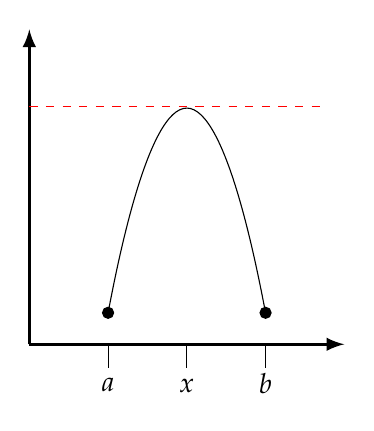
\begin{tikzpicture}[scale = 2]
        \draw[-latex, very thick] (0, 0) -- (0, 2);
        \draw[-latex, very thick] (0, 0) -- (2, 0);
        \draw[] (1, 1.5) parabola (0.5, 0.2);
        \draw[] (1, 1.5) parabola (1.5, 0.2);
        \filldraw[] (0.5, 0.2) circle (1pt);
        \filldraw[] (1.5, 0.2) circle (1pt);
        \draw[dashed, red] (0, 1.51) -- (1.85, 1.51);
        \draw[] (0.5, 0) -- (0.5, -0.15);
        \node[below] at (0.5, -0.15) {$a$};
        \draw[] (1.5, 0) -- (1.5, -0.15);
        \node[below] at (1.5, -0.12) {$b$};
        \draw[] (1, 0) -- (1, -0.15);
        \node[below] at (1, -0.16) {$x$};
    \end{tikzpicture}
    
    \caption{A simple parabolic function that demonstrates Rolle's Theorem.}
    \label{fig21}
\end{figure}

\newpage 
\setcounter{rudin}{9}
\begin{theorem}{Mean Value Theorem}{5.10}
    Let $f: [a, b] \mapsto \RR$ be continuosu and differentiable on $(a, b)$. Then, there exists $x \in (a, b)$ such that $f(b) - f(a) = f'(x)(b - a)$.
\end{theorem}
\noindent The visual interpretation of this theorem is that there exists $x \in (a, b)$ such that the slope of the tangent line to $f$ at $x$ is equal to the secant line slope between $(a, f(a))$ and $(b, f(b))$. The idea of the proof is to rotate one's head such that the sectant line is horizontal; one is then able to apply Rolle's Theorem!

\begin{nproof}
    Define $h(y) = f(y) = \frac{f(b) - f(a)}{b - a}(y - a)$. $h$ is continuous on $[a, b]$ and differentiable on $(a, b)$ (being a sum of continuous/differentiable functions). We have that $h(a) = f(a) - 0 = f(a)$, and $h(b) = f(b) - \frac{f(b) - f(a)}{b - a}(b - a) = f(a)$. Applying Rolle's Theorem to $h$, there exists $x \in (a, b)$ such that $h'(x) = 0$. Therefore, $h'(x) = 0 = f'(x) - \frac{f(a) - f(b)}{b - a} = 0$, and we conclude that $f(b) - f(a) = f'(x)(b - a)$ for some $x \in (a, b)$. \qed
\end{nproof}

\begin{figure}[htbp]
    \centering
    \begin{tikzpicture}[scale=2]
    \draw[-latex, very thick] (0, 0) -- (0, 2);
    \draw[-latex, very thick] (0, 0) -- (2, 0);
    \draw [] (0.5 , 0.25) to [ curve through ={(1, 1.25)}] (1.5,1.5);
    \filldraw[] (0.5, 0.25) circle (1pt);
    \filldraw[] (1.5, 1.5) circle (1pt);
    \draw[dashed] (0.5, 0.25) -- (1.5, 1.5);
    \draw[dashed, red] (0, 0.075) -- (1, 1.325) -- (1.42,1.85);
    \draw[] (0.5, 0) -- (0.5, -0.15);
    \node[below] at (0.5, -0.15) {$a$};
    \draw[] (1.5, 0) -- (1.5, -0.15);
    \node[below] at (1.5, -0.12) {$b$};
    \draw[] (0.775, 0) -- (0.775, -0.15);
    \node[below] at (0.775, -0.16) {$x$};
    \end{tikzpicture}
    \caption{A simple continuous function that demonstrates the MVT.}
    \label{fig22}
\end{figure}


\begin{theorem}{}{5.11}
    Let $f: [a, b] \mapsto \RR$ be differentiable on $(a, b)$. Then:
    \begin{enumerate}
        \item If $f'(x) \geq 0$ for all $x \in (a, b)$, then $f$ is monotonically increasing.
        \item If $f'(x) = 0$ for all $x \in (a, b)$, then $f$ is constant. 
        \item If $f'(x) \leq 0$ for all $x \in (a, b)$, then $f$ is monotonically decreasing.
    \end{enumerate} 
\end{theorem}
\begin{nproof}
    If $a < x < y < b$, by the mean value theorem, there exists $z \in (x, y)$ such that:
    \begin{align*}
        f(y) - f(x) = f'(z)(y - x)
    \end{align*}
    Note that $y - x > 0$ by construction. 
    \begin{enumerate}
        \item If $f'(x) \geq 0$ for all $x \in (a, b)$, then $f'(z) \geq 0$, showing that $f(y) - f(x) \geq 0$ and hence that $f$ is monotonically increasing. 
        \item If $f'(x) = 0$ for all $x \in (a, b)$, then $f'(z) = 0$, showing that $f(y) - f(x) = 0$ and hence that $f$ is constant on $(a, b)$.
        \item If $f'(x) \leq 0$ for all $x \in (a, b)$, then $f'(z) \leq 0$, showing that $f(y) - f(x) \leq 0$ and hence that $f$ is monotonically decreasing. \qed
    \end{enumerate}
\end{nproof}

\subsection{Taylor's Theorem}
\setcounter{rudin}{13}
\begin{definition}{Higher Order Derivatives}{5.14}
If $f$ is differentiable in a neighbourhood of $x$, then we may compute a second order derivative:
\begin{align*}
    \lim_{t \rightarrow x} \frac{f'(t) - f'(x)}{t - x} = (f')'(x) = f''(x)
\end{align*}
We can then continue this process to obtain $f^{(3)}(x), f^{(4)}(x), \ldots, f^{(n)}(x)$. 
\end{definition}
\begin{ndef}{: \texorpdfstring{$C^n(I, \RR)$}{Cn(I, R)}}{}
    If $f$ is continuous in $I$, we can write $f \in C^{0}(I, \RR)$. If $f$ is differentiable in a neighbourhood $I$ and the derivative $f'$ is continuous in $I$, then we write $f \in C^{1}(I, \RR)$. In general, $f \in C^{n}(I, \RR)$ denotes the $n$th derivative of $f$ is continuous in $I$. Note that where it is clear from context, we may drop the $\RR$ and just write $C^n(I)$. 
\end{ndef}
\noindent Recall that for a function $f$ continuous and differentiable on $(x_0, x)$, the Mean Value Theorem proved the existence of some $\tilde{x}$ such that:
\begin{align*}
    f(x) = f(x_0) + f'(\tilde{x})(x - x_0)
\end{align*}
This gives us a natural method to build up approximations for functions; we can start with a constant approximation $f(x_0)$, then add a linear term $f'(\tilde{x})(x - x_0)$, then add on a quadratic term $(x - x_0)^2$ and so on. The following theorem gives us a way to construct these approximations and bound their error.

\begin{theorem}{Taylor's Theorem}{5.15}
    Let $I$ be a neighbourhood of $x_0$, and $f \in C^p(I)$. Then, for any $n < p$, we have that:
    \begin{align*}
        f(x) = \sum_{j=0}^n \frac{f^{(j)}(x_0)}{j!}(x- x_0)^j + \frac{f^{(n+1)}(\tilde{x})}{(n+1)!}(x - x_0)^{n+1}
    \end{align*}
    Where $\tilde{x} = x_0 + \lambda(x - x_0)$ for some $\lambda \in (0, 1)$ (i.e. $\tilde{x} \in (x_0, x)$). Note that $\tilde{x}$ depends on $x, x_0$, and $n$. 
\end{theorem}
\begin{nproof}
    For $n = 0$, the claim reduces to the Mean Value Theorem. Then, let $n \geq 1$. Let $A$ be a constant that depends on $x, x_0$, and $n$, and let $P_n(x) = \sum_{j=0}^n \frac{f^{(j)}(x_0)}{j!}(x-x_0)^j$. Then, we can write:
    \begin{align*}
        f(x) = P_n(x) + A(x-x_0)^{n+1}
    \end{align*}
    We need to show that we can express $A$ as relating to the derivative, namely, that there exists $\tilde{x}$ such that $A = \frac{f^{(n+1)}(\tilde{x})}{(n+1)!}$. Let $g(t) = f(t) - P_n(t) - A(t - x_0)^{n+1}$ with $t \in I$. Then, $g \in C^{p}(I)$. For $n < p$, we then have that:
    \begin{align*}
        g^{(n+1)}(t) = f^{(n+1)}(t) - 0 - A(n+1)!(t - x_0)
    \end{align*}
    We claim that there exists $\tilde{x} \in (x_0, x)$ such that $g^{(n+1)}(\tilde{x}) = 0$. To see this, consider that $P^{(j)}(x_0) = f^{(j)}(x_0)$ for $j = 0, 1, \ldots, n$, so $g(x_0) = 0$, and furthermore:
    \begin{align*}
        g'(x_0) = g''(x_0) = g^{(3)}(x_0) = \ldots = g^{(n)}(x_0) = 0
    \end{align*}
    Moreover y the choice of $n$, we have that $g(x) = 0$. Hence, by Rolle's Theorem, there exists a point $x_1$ between $x_0$ and $x$ such that $g'(x_1) = 0$. Similarly, repeating the argument above, there exists an $x_2$ between $x_0$ and $x_1$ such that $g''(x_2) = 0$. Repeating this process up to $g^{(n)}$, we have that $g^{(n)}(x_n) = 0$, for some $x_0 < x_{n} < x_{n-1} < \cdots < x$ and in turn, there exists $x_{n+1} \in (x_0, x_n)$ such that $g^{(n+1)}(x_{n+1}) = 0$. Setting $\tilde{x} = x_{n+1}$, the claim is shown. \qed
\end{nproof}

\noindent As an example, we consider the Taylor series of the function $f(x) = \cos(x)$ (We will formally define this function later on, but for now, let us assume its familar properties and derivatives). We then have that:
\begin{align*}
    f^{(j)}(0) = \begin{cases}
        (-1)^m & \text{if $j = 2m$}
        \\ 0 & \text{if $j = 2m + 1$}
    \end{cases}
\end{align*}
If we have the sum run from $j = 0$ to some $j = n$, let us then try to estimate the rest. Let $\tilde{x} \in (0, x)$. Then, letting the error term be represented by $\e$, we have that:
\begin{align*}
    \e = \abs{\frac{f^{(n+1)}(\tilde{x})}{(n+1)!}(x-x_0)^{n+1}} \leq \frac{\abs{x}^{n+1}}{(n+1)!} 
\end{align*}
And we observe that $\linf \frac{\abs{x}^{n+1}}{(n+1)!} = 0$ and hence the error $\e$ goes to zero in the $n \rightarrow \infty$ limit. Therefore, the difference between $\cos(x)$ and its Taylor polynomial vanishes quickly for any $x$, and the Taylor series converges for all $x$. Taking the limit of the sum, we have that:
\begin{align*}
    f(x) = \cos(x) = \linf \left(P_{n}(x) + \frac{f^{(n+1)}(x_0)}{(n+1)!}(x - x_0)^{n+1}\right) = \sum_{j=0}^\infty \frac{(-1)^{2m}}{m!}x^{2m} = 1 - \frac{x^2}{2} + \frac{x^4}{4} - \frac{x^6}{6} + \ldots
\end{align*}
A question of interest might be how many terms do we need in the Polynomial such that our error is less than $10^{-6}$, say, for estimating the value of $\cos(\frac{\pi}{12})$. In other words, we want to find the $m$ such that:
\begin{align*}
    \frac{1}{2m!}\left(\frac{\pi}{12}\right)^{2m} \leq 10^{-6}
\end{align*}
Rearranging, we require:
\begin{align*}
    (2m)!\left(\frac{12}{\pi}\right)^{2m} > 10^6
\end{align*}
Making a table of the value of the LHS as a function of $m$, we have:
\begin{table}[htbp]
    \centering\begin{tabular}{c|c}
    $m$ & $(2m)!\left(\frac{12}{\pi}\right)^{2m}$
    \\ \hline
    1 & $\approx 29$
    \\ 2 & $\approx 5110$
    \\ 3 & $\approx 2.23 \times 10^{6}$
    \end{tabular}
\end{table}
So we see that three terms are sufficient for a good approximation in this case (and as stated before, the series converges very quickly)!

A natural question of interest is the convergence of the sum in the $N \rightarrow \infty$ limit, that is, the convergence of the power series $\sum_{n = 0}^\infty \frac{f^{(n)}(x_0)}{n!}(x - x_0)^n$. We are also interested are interested for when $f(x) = \sum_{n = 0}^\infty \frac{f^{(n)}(x_0)}{n!}(x - x_0)^n$ holds (that is, when is a function equal to its Taylor series)? These turn out to be distinct questions; in particular, there are functions whose power series converge for all $x$ but are equal to their power series nowhere (except at $x_0$ where equality must hold). This motivates the following definition:
\begin{ndef}{: Analyticity}{}
    A function $f$ is \textbf{analytic} if $f(x) = \sum_{n=0}^\infty \frac{f^{(n)}(x_0)}{n!}(x - x_0)^n$ in a neighbourhood of $x_0$.
\end{ndef}
\noindent To motivate this definition, it will help to study a function which is \textit{not} analytic. Consider the function:
\begin{align*}
    f(x) = \begin{cases}
        \exp(-\frac{1}{x}) & x > 0
        \\ 0 & x \leq 0
    \end{cases}
\end{align*}
\begin{figure}[htbp]
    \centering
    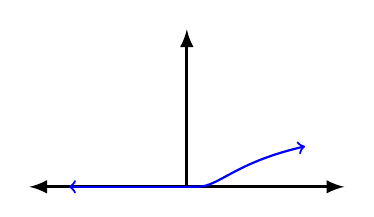
\begin{tikzpicture}
        \draw[latex-latex, very thick] (-2, 0) -- (2, 0);
        \draw[-latex, very thick] (0, 0) -- (0, 2);
        \draw[<-, blue, thick] (-1.5, 0) -- (0.02, 0);
        \draw[->, blue, thick, smooth, samples = 100, domain=0.01:1.5, variable = \x] plot(\x, {exp(-1/\x)});
    \end{tikzpicture}
    \caption{Plot of $f$.}
    \label{fig23}
\end{figure}

\noindent $f$ is continuous everywhere by construction. It is infinitely differentiable at $x = 0$, but it is only equal to its Taylor series around $x_0 =0$ for $x \leq 0$. To see this, we observe that:

\begin{align*}
    f'(x) = \frac{1}{x^2}\exp(-\frac{1}{x})
\end{align*}
\begin{align*}
    f^{(n)}(x) = \frac{P_n(x)}{x^{2n}}\exp(-\frac{1}{x})
\end{align*}
We have that $f^{(n)}(x) \rightarrow 0$ as $x \rightarrow 0$ for all $n$ as the exponential dominates the polynomial singularity. We hence have that $f \in C^\infty$. The taylor polynomial at $x_0 = 0$ however, as we have that $f(0) = 0$ and $f^{(n)}(0) = 0$, leading to:
\begin{align*}
    \sum_{n=0}^N \frac{f^{(n)}(0)}{n!}x^n = 0
\end{align*}
for all $N$. We therefore have that the series converges for all $x$, but is only equal to $f$ for $x \leq 0$; hence it is not analytic (as there exists no neighbourhood around $x_0= 0$ for which $f$ is equal to its Taylor series). 

We now consider a function $\chi(x)$ defined as $\chi(x) = \frac{f(x)}{f(x) + f(1 - x)}$. This function is alsoz continuous, its denominator is never zero, and $\chi \in C^\infty$. We observe that $\chi(x) = 0$ for $x \leq 0$ and $\chi(x) = 1$ for $x \geq 1$, and overall the function looks much like a step function:

\begin{figure}[htbp]
    \centering
    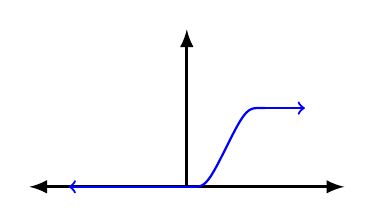
\begin{tikzpicture}
        \draw[latex-latex, very thick] (-2, 0) -- (2, 0);
        \draw[-latex, very thick] (0, 0) -- (0, 2);
        \draw[<-, blue, thick] (-1.5, 0) -- (0.02, 0);
        \draw[blue, smooth, samples = 100, domain=0.01:0.99, variable = \x, thick] plot(\x, {exp(-1/\x)/(exp(-1/\x) + exp(-1/(1-\x)))});
        \draw[blue, ->, thick] (0.98, 1) -- (1.5, 1);
    \end{tikzpicture}
    \caption{Plot of $\chi$.}
    \label{fig24}
\end{figure}
Indeed, this function can be used as a ``cutoff''/``switch'' function that behaves much like a step function (except it is infinitely differentiable).

A question becomes whether such a function could be analytic. The answer turns out to be no, and the proof we leave as an exercise. As a sketch, consider an analytic function $g$ such that $g(x) = 0$ for $x \leq x_0$ and $g(x) \neq 0$ for $x > x_0$. One can derive a contradiction by considering the Taylor series expansion about $x_0$ and then using the assumed analyticity of $g$. 

Note that in a sense, Taylor's Theorem is the culmination of a sequence of theorems we have proven in the course. Roughly, the sequence was as follows:
\begin{enumerate}[1)]
    \item $f: X \mapsto Y$ and $K \subset X$, then $f(K)$ compact (Theorem \ref{thm:4.14})
    \item Extreme Value Theorem: If $f: X \mapsto \RR$ with $f$ continu$(X, \tau)$ and $(Y, \rho)$ ous and $K$ compact, then $f$ realizes its supremum and infimum on $K$. (Theorem \ref{thm:4.16})
        
    \item Rolle's Theorem
    \item Mean Value Theorem (Theorem \ref{thm:5.10})
    \item Taylor's Theorem (Theorem \ref{thm:5.15})
\end{enumerate}
A question that arises is could we have gone through this sequence of proofs with just the rational numbers ($\QQ$)? The intuitive answer is no, but it may be interesting to see where along this chain the logic breaks down.

The first step that looks immediately questionable is step 2; the supremum/infimum is not well-defined for all subsets of $\QQ$, so we might be able to find a breakdown there. To this end, we consider the set $A = \set{q \in \QQ: q > 0, q^2 < 2}$ that arises in Example \ref{exam:1.1a} and try to find a function $f: K \mapsto \QQ$ with $K \subset \QQ$ compact such that $f(K) = A$. An idea would be to try $f(x) = \sqrt{x}$, with $K = \set{q \in \QQ: \exists r: r^2 = q} \cap [0, 2]$ but this doesn't work as $K$ is not compact. Trying another attempt, $K = [1, 2] \cap \QQ$ with $f(x) = \sin(x)$ does not work either as $\sin(x)$ is not necessarily rational, and moreover, $[1, 3] \cap \QQ$ is not a compact set as not all Cauchy sequences in $S$ converge! Another attempt would be $K = [1, 2] \cap \QQ = X$ with $f(q) = \abs{q^2 - 2}$ where it would seem as though $f(K) = \set{r \in \QQ: 0 < r \leq 2}$ provides a good counterexample, but this fails for the same reason as $K$ is not compact. Finding a valid counterexample for the EVT is therefore difficult. 

An easier break along the chain to find is with Rolle's Theorem. One can consider the function $f(x) = x^2 - 2$ which can break the Intermediate value theorem as $0$ is not contained in the image if the domain is $\QQ$. We can dress this up to construct a counterexample for Rolle's Theorem.

\subsection{Local Behavior of Functions}
\begin{ntheorem}{: Second Derivative Test}{}
    Suppose $f \in C^{3}(I)$ where $I$ is a neighbourhood of $x_0$. Furthermore, suppose that $f'(x_0) = 0$. If $f''(x_0) > 0$, then $x_0$ is a local minimum. Conversely, if $f''(x_0) < 0$, then $x_0$ is a local maximum.
\end{ntheorem}
\begin{nproof}
    By Taylor's Theorem (Theorem \ref{thm:5.15}), if we let $x = x_0 + h$ for $h > 0$, there exists some $\tilde{x} = x_0 + \lambda h$ with $\lambda \in (0, 1)$ such that:
    \begin{align*}
        f(x) = f(x_0) + f'(x_0)(x - x_0) + \frac{1}{2}f''(x_0)(x - x_0)^2 + \frac{1}{6}f^{(3)}(\tilde{x})(x - x_0)^3
    \end{align*}
    Using that $f'(x_0) = 0$, we have:
    \begin{align*}
        f(x) - f(x_0) = h^2\left(\frac{1}{2}f''(x_0) + \frac{1}{6}f^{(3)}(x_0 + \lambda h) h\right)
    \end{align*} 
    Let $0 < \e < \abs{\frac{1}{2}f''(x_0)}$. Then, by the assumed continuity of $f^(3)$, we have that there exists $\delta > 0$ such that $\abs{h} < \delta$ implies $\abs{\frac{1}{6}f^{(3)}(x_0 + \lambda h)h} < \e$. Hence, for sufficiently small $h$, we have that:
    \begin{align*}
        \sgn\left(f(x) - f(x_0)\right) = \sgn(f''(x_0))
    \end{align*}
    So we conclude that if $f'(x_0) = 0$ and $f''(x_0) > 0$ then $x_0$ is a local minimum, and if $f''(x_0) < 0$, then $x_0$ is a local maximum. \qed
\end{nproof}

\begin{ndef}{: Convex Functions}{}
    Let $f: (a, b) \mapsto \RR$ is \textbf{convex} if for all $x, y \in (a, b)$ with $a < x < y < b$ and for all $\lambda \in (0, 1)$,
    \begin{align*}
        f(\lambda x + (1 - \lambda)y) \leq \lambda f(x) + (1 - \lambda)f(y)
    \end{align*}
\end{ndef}
\noindent Note that an alternative definition of convexity is that for any $x, y$ with $x < y$, the function evaluated at some point $z \in (x, y)$ will always be below the average of the function at $x, y$. That is:
\begin{align*}
    f(z) \leq \frac{f(x) + f(y)}{2}
\end{align*}
\begin{figure}[htbp]
    \centering
    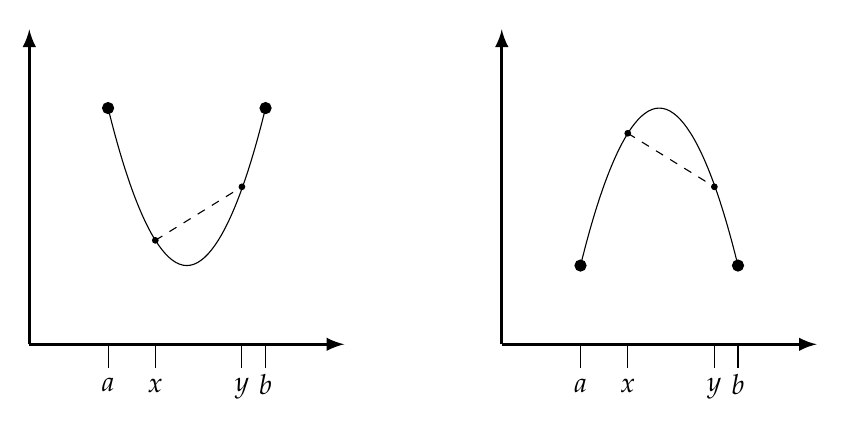
\begin{tikzpicture}[scale=2]
        \draw[-latex, very thick] (-2.5, 0) -- (-2.5, 2);
        \draw[-latex, very thick] (-2.5, 0) -- (-0.5, 0);
        \draw[] (-1.5, 0.5) parabola (-2, 1.5);
        \draw[] (-1.5, 0.5) parabola (-1, 1.5);
        \filldraw[] (-2, 1.5) circle (1pt);
        \filldraw[] (-1, 1.5) circle (1pt);
        \draw[] (-2, 0) -- (-2, -0.15);
        \node[below] at (-2, -0.15) {$a$};
        \draw[] (-1, 0) -- (-1, -0.15);
        \node[below] at (-1, -0.13) {$b$};
        \draw[] (-1.7, 0) -- (-1.7, -0.15);
        \node[below] at (-1.7, -0.16) {$x$};
        \draw[] (-1.15, 0) -- (-1.15, -0.15);
        \node[below] at (-1.15, -0.15) {$y$};
        \filldraw[] (-1.7, 0.66) circle (0.5pt);
        %\node[left] at (-2.5, 0.66) {$f(x)$};
        \filldraw[] (-1.15, 1) circle (0.5pt);
        %\node[left] at (-2.5, 1) {$f(y)$};
        \draw[dashed] (-1.7, 0.66) -- (-1.15, 1);
        \draw[-latex, very thick] (0.5, 0) -- (0.5, 2);
        \draw[-latex, very thick] (0.5, 0) -- (2.5, 0);
        \draw[] (1.5, 1.5) parabola (1, 0.5);
        \draw[] (1.5, 1.5) parabola (2, 0.5);
        \filldraw[] (1, 0.5) circle (1pt);
        \filldraw[] (2, 0.5) circle (1pt);
        \draw[] (1, 0) -- (1, -0.15);
        \node[below] at (1, -0.16) {$a$};
        \draw[] (2, 0) -- (2, -0.15);
        \node[below] at (2, -0.13) {$b$};
        \draw[] (1.3, 0) -- (1.3, -0.15);
        \node[below] at (1.3, -0.16) {$x$};
        \draw[] (1.85, 0) -- (1.85, -0.15);
        \node[below] at (1.85, -0.15) {$y$};
        \filldraw[] (1.3, 1.34) circle (0.5pt);
        \filldraw[] (1.85, 1) circle (0.5pt);
        \draw[dashed] (1.3, 1.34) -- (1.85, 1);
    \end{tikzpicture}
    \caption{Visualization of a convex and non-convex function. For the upwards facing parabola, the function (and hence all points $(\lambda x + (1- \lambda) y, f(\lambda x + (1- \lambda) y))$ for $\lambda \in (0, 1)$) always lies below the line connecting $(x, f(x))$ and $(y, f(y))$ for $a < x < y < b$ and hence it is convex. For the downwards facing parabola, this is no longer true and the function is not convex (it is instead\textit{concave}).}
    \label{fig25}
\end{figure}

\noindent Another equivalent way of defining convexity is to say that $f$ is convex if and only if for all $a < s < t < y < b$:
\begin{align*}
    \frac{f(t) - f(s)}{t - s} \leq \frac{f(u) - f(t)}{u - t}
\end{align*}

\begin{figure}[htbp]
    \centering
    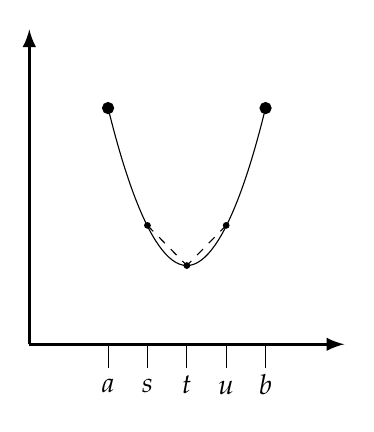
\begin{tikzpicture}[scale=2]
        \draw[-latex, very thick] (0, 0) -- (0, 2);
        \draw[-latex, very thick] (0, 0) -- (2, 0);
        \draw[] (1, 0.5) parabola (0.5, 1.5);
        \draw[] (1, 0.5) parabola (1.5, 1.5);
        \filldraw[] (0.5, 1.5) circle (1pt);
        \filldraw[] (1.5, 1.5) circle (1pt);
        \draw[] (0.5, 0) -- (0.5, -0.15);
        \node[below] at (0.5, -0.16) {$a$};
        \draw[] (1.5, 0) -- (1.5, -0.15);
        \node[below] at (1.5, -0.13) {$b$};
        \draw[] (0.75, 0) -- (0.75, -0.15);
        \node[below] at (0.75, -0.16) {$s$};
        \draw[] (1.25, 0) -- (1.25, -0.15);
        \node[below] at (1.25, -0.17) {$u$};
        \draw[] (1, 0) -- (1, -0.15);
        \node[below] at (1, -0.14) {$t$};
        \filldraw[] (1, 0.5) circle (0.5pt);
        \filldraw[] (0.75, 0.755) circle (0.5pt);
        \filldraw[] (1.25, 0.755) circle (0.5pt);
        \draw[dashed] (0.75, 0.755) -- (1, 0.5);
        \draw[dashed] (1.25, 0.755) -- (1, 0.5);
    \end{tikzpicture}
    
    \caption{Visualization of the alternative definition of convexity. For any $a < s < t < u < v$, the slope of the line segment joining $s$ and $t$ is less than the slope of the line segment joining $t$ and $u$.}
    \label{fig26}
\end{figure}

\begin{ntheorem}{}{}
    \begin{enumerate}[(a)]
        \item Assume that $f: (a, b) \mapsto \RR$ is convex. Then, $f$ is continuous.
        \item Assume that $f \in C^1(a, b)$. Then, if $f$ is convex, $f'$ is increasing.
        \item Assume that $f \in C^2(a, b)$. Then $f$ convex implies $f'' \geq 0$. 
    \end{enumerate}
\end{ntheorem}
\begin{nproof}
    \begin{enumerate}
        \item Let $[c, d] \subset (a, b)$ and $a < c_1 < c < x < y < d < d_1 < b$. By convexity, we have that:
        \begin{align*}
            \frac{f(y) - f(x)}{y - x} \leq \frac{f(d) - f(y)}{d - y} \leq \frac{f(d_1) - f(d)}{d_1 - d}
        \end{align*}
        and also that:
        \begin{align*}
            \frac{f(y) - f(x)}{y - x} \geq \frac{f(x) - f(c)}{x - c} \geq \frac{f(c) - f(c_1)}{c - c_1}
        \end{align*}
        We therefore have that:
        \begin{align*}
            \set{\abs{\frac{f(y) - f(x)}{y - x}}: c < x < y < b} < M
        \end{align*}
        for some $M \in \RR$. Therefore, $\abs{f(y) - f(x)} < M\abs{y - x}$ for all $x, y \in (c, d)$. This holds for all $[c, d] \subset (a, b)$, showing the continuity of $f$.
        \item Let $f$ be convex, and let $a < c < x < y < d < b$. Then, by convexity we have that:
        \begin{align*}
            \frac{f(x) - f(c)}{x - c} \leq \frac{f(y) - f(x)}{y - x} \leq \frac{f(d) - f(y)}{d - y}
        \end{align*}
        Ignoring the central term in the inequality, and taking the limit as $x \rightarrow c$ and $ y \rightarrow b$, we have that:
        \begin{align*}
            f'(c) \leq f'(b)
        \end{align*}
        So we conclude that $f'$ is increasing on $(a, b)$. 
        \item If $f$ is convex, $f'$ is increasing by (b). Then, we have that for any $a < x < y < b$:
        \begin{align*}
            \frac{f(y) - f(x)}{y - x} \geq 0
        \end{align*}
        And hence taking $y \rightarrow x$ we have that $f'(x) \geq 0$. \qed
    \end{enumerate}
\end{nproof}

\begin{ncorollary}{}{}
    If $f \in C^3(I)$ and $f'(x_0) = 0$ and $f''(x_0) \neq 0$, $x_0$ is a local minimum if $f$ is convex in a neighbourhood of $x_0$. 
\end{ncorollary}
\section{The Riemann-Stieltjes Integral}
\section[Sequences and Series of Functions]{\hyperlink{toc}{Sequences and Series of Functions}}

\subsection{Motivating Examples}
\begin{nexample}{}{}
    For $m, n \in \NN$, let $p_{n, m} = \frac{m}{n}$. Then, 
    \begin{align*}
        \lim_{m\rightarrow \infty} p_{m, n} = \infty, \quad \linf p_{m, n} = 0
    \end{align*}
    In particular,
    \begin{align*}
        \lim_{m \rightarrow \infty}\linf p_{m, n} = 0, \quad \linf\lim_{m \rightarrow \infty} p_{m, n} = \infty.
    \end{align*}
    Which demonstrates that the order of which limits are taken in can affect the value.
\end{nexample}

\begin{nexample}{}{}
    Define the sequence of functions:
    \begin{align*}
        f_n(x) = \begin{cases}
            1 & x \geq 0
            \\ 1 + nx & -\frac{1}{n} < x < 0
            \\ 0 & x \leq -\frac{1}{n}
        \end{cases}
    \end{align*}
    Since $f_n$ is piecewise linear, it is continuous. However, looking at the $n \rightarrow \infty$ limit, we have:
    \begin{align*}
        \linf f_n(x) = \begin{cases}
            1 & x \geq 0
            \\ 0 & x < 0
        \end{cases}
    \end{align*}
    Which is the right continuous step function, which is evidently discontinuous at $x = 0$. Hence, the limit of continuous functions can be discontinuous. Another way of viewing this problem is:
    \begin{align*}
        \linf \lim_{x \rightarrow 0} f_n(x) = 0, \quad \lim_{x \rightarrow 0} \linf f_n(x) = \text{D.N.E.}
    \end{align*}
    so again we see the order of taking our limits can be important.
\end{nexample}
\begin{figure}[htbp]
    \centering
    \begin{tikzpicture}[scale=1.5]
        \draw[latex-latex, very thick] (-2, 0) -- (2, 0);
        \draw[-latex , very thick] (0, 0) -- (0, 2);
        \draw[<-, thick, blue] (-1.5, 0) -- (-0.5, 0);
        \draw[thick, blue] (-0.5, 0) -- (0, 1);
        \draw[->, thick, blue] (0,1) -- (1.5, 1);
        \draw[] (-0.5, 0) -- (-0.5, -0.15);
        \node[below] at (-0.5, -0.15) {$-\frac{1}{n}$};
    \end{tikzpicture}
    
    
    \caption{Plot of $f_n$ in the above example.}
    \label{fig37}
\end{figure}

\setcounter{rudin}{3}

\begin{example}{}{7.4}
    For $m \in \NN$ and $x \in \RR$, let $f_m(x) = \lim_{n \rightarrow \infty} \left[\cos(m!\pi x)\right]^{2n}$. Since $\abs{\cos(k\pi)} = 1$ if $k \in \ZZ$, we see that $f_m(x) = 1$ when $m! x \in \ZZ$. Conversely, since $\abs{\cos(k\pi)} < 1$ if $k \neq \ZZ$, $f_m(x) = 0$ when $m! x \notin \ZZ$. Some plots of $f_m(x)$ on $[0, 1]$ for $m = 1, 2, 3$ are below as a visualization. We now define $f(x) = \lim_{m \rightarrow \infty} f_m(x)$. If $x = \frac{p}{q} \in \QQ$, then $m! x = \frac{m! p}{q} \in \ZZ$ for $m$ large enough (for $m \geq q$, as the denominator cancells). Therefore, we have that $f(x) = 1$ for $x \in \QQ$. Conversely, if $x \notin \QQ$, then $m! x \notin \ZZ$ for all $m \in \NN$. So, $f_m(x) = 0$ for all $m$, and $f(x) = 0$. Therefore, we have that:
    \begin{align*}
        f(x) = \lim_{m \rightarrow \infty} f_m(x) = \begin{cases}
            1 & x \in \QQ
            \\ 0 & x \notin \QQ
        \end{cases}.
    \end{align*}
    In other words, $f$ is the Dirchlet function. The interesting part is that each of the $f_m(x)$ are Riemann integrable on $[0, 1]$ by Theorem \ref{thm:6.10} (as $f$ has finitely many discontinuities for any $m \in \NN$). However, the limit is not Riemann integrable, as we prove below. Hence, the limit of Riemann integrable functions is not necessarily Riemann integrable.
\end{example}

\begin{figure}[htbp]
    \centering
    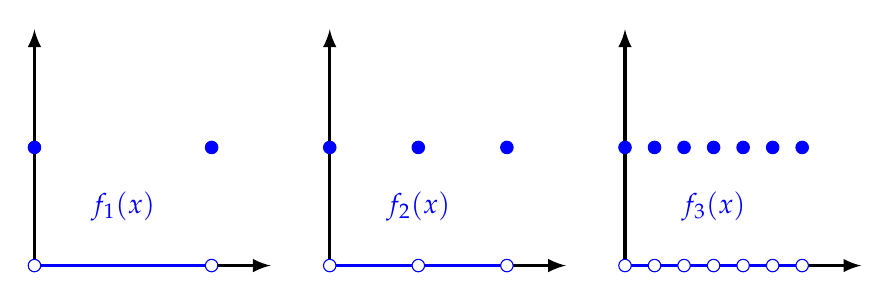
\begin{tikzpicture}[scale = 1.5]
        \draw[-latex, very thick] (0, 0) -- (0, 2);
        \draw[-latex, very thick] (0, 0) -- (2, 0);
        \draw[-latex, very thick] (2.5, 0) -- (2.5, 2);
        \draw[-latex, very thick] (2.5, 0) -- (4.5, 0);
        \draw[-latex, very thick] (5, 0) -- (5, 2);
        \draw[-latex, very thick] (5, 0) -- (7, 0);
        \filldraw[blue] (0, 1) circle (1.5pt);
        \filldraw[blue] (1.5, 1) circle (1.5pt);
        \draw[thick, blue] (0, 0) -- (1.5, 0);
        \draw[blue, fill = white] (0, 0) circle (1.5pt);
        \draw[blue, fill = white] (1.5, 0) circle (1.5pt);
        \node[text = blue] at (0.75, 0.5) {$f_1(x)$};

        \filldraw[blue] (2.5, 1) circle (1.5pt);
        \filldraw[blue] (3.25, 1) circle (1.5pt);
        \filldraw[blue] (4, 1) circle (1.5pt);
        \draw[thick, blue] (2.5, 0) -- (4, 0);
        \draw[blue, fill = white] (2.5, 0) circle (1.5pt);
        \draw[blue, fill = white] (3.25, 0) circle (1.5pt);
        \draw[blue, fill = white] (4, 0) circle (1.5pt);
        \node[text = blue] at (3.25, 0.5) {$f_2(x)$};

        \filldraw[blue] (5, 1) circle (1.5pt);
        \filldraw[blue] (5.25, 1) circle (1.5pt);
        \filldraw[blue] (5.5, 1) circle (1.5pt);
        \filldraw[blue] (5.75, 1) circle (1.5pt);
        \filldraw[blue] (6, 1) circle (1.5pt);
        \filldraw[blue] (6.25, 1) circle (1.5pt);
        \filldraw[blue] (6.5, 1) circle (1.5pt);
        \draw[thick, blue] (5, 0) -- (6.5, 0);
        \draw[blue, fill = white] (5, 0) circle (1.5pt);
        \draw[blue, fill = white] (5.25, 0) circle (1.5pt);
        \draw[blue, fill = white] (5.5, 0) circle (1.5pt);
        \draw[blue, fill = white] (5.75, 0) circle (1.5pt);
        \draw[blue, fill = white] (6, 0) circle (1.5pt);
        \draw[blue, fill = white] (6.25, 0) circle (1.5pt);
        \draw[blue, fill = white] (6.5, 0) circle (1.5pt);
        \node[text = blue] at (5.75, 0.5) {$f_3(x)$};
    \end{tikzpicture}
    \caption{Plot of $f_m(x)$ over the interval $[0, 1]$ for $m = 1, 2, 3$. For $m = 1$, only $x = 0, 1$ satisfy $m! x = x \in \ZZ$. For $m = 2$, we have that $x = 0, \frac{1}{2}, 1$ satisfy $m!x = 2x \in \ZZ$. Finally, for $m = 3$, we have that $x = 0, \frac{1}{6}, \frac{2}{6}, \frac{3}{6}, \frac{4}{6}, \frac{5}{6}, 1$ satisfy $m!x = 6x \in \ZZ$.}
    \label{fig38}
\end{figure}

\noindent We now show that $f$ defined in the above example is not Riemann integrable on $[0, 1]$.

\begin{proof}
    Consider any partition $P$ of $[0, 1]$. Due to the density of rational and irrational numbers in $\RR$ (Theorem \ref{thm:1.20}) we have that $M_i = \sup{f(x): x \in [x_{i-1}, x_i]} = 1$ and $m_i = \inf{f(x): x \in [x_{i-1}, x_i]} = 0$ for all $i$. Therefore, we have that $U(P, f) = \sum_{i=1}^N M_i \Delta x_i = 1$ and $L(P, f) = \sum_{i=1}^N m_i \Delta x_i = 0$ for all partitions $P$. Therefore, $\sup_P U(P, f) = 1$ and $\inf_P L(P, f) = 0$, and we conclude that $f$ is not Riemann integrable on $[0, 1]$.
\end{proof}


\begin{nexample}{}{}
    Define $f_n$ such that:
    \begin{align*}
        f_n(x) = \begin{cases}
            0 & \abs{x} \geq \frac{1}{n}
            \\ n(nx+1) & -\frac{1}{n} < x < 0
            \\ -n(nx+1) & 0 < x < \frac{1}{n}
            \\ 0 & x = 0
        \end{cases}
    \end{align*}
    Then, we have that $f(x) = \linf f_n(x) = 0$ for all $x$.  Furthermore, we have that $\int_{-1}^1 f_n(x)dx = 1$ for all $n$, but $\int_{-1}^1 f(x)dx = 0$. Hence, we have that:
    \begin{align*}
        \linf \int_{-1}^1 f_n(x)dx = 1 \neq 0 = \int_{-1}^1 \linf f_n(x) dx
    \end{align*}
    showing that problems can arise when we interchange the order of an integral with a limit.
\end{nexample}

\begin{figure}[htbp]
    \centering
    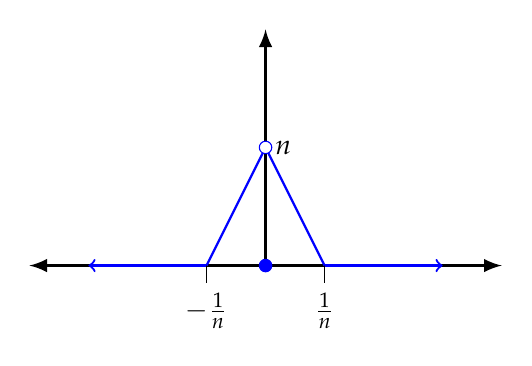
\begin{tikzpicture}[scale=1.5]
        \draw[latex-latex, very thick] (-2, 0) -- (2, 0);
        \draw[-latex , very thick] (0, 0) -- (0, 2);
        \draw[<-, thick, blue] (-1.5, 0) -- (-0.5, 0);
        \draw[thick, blue] (-0.5, 0) -- (0, 1);
        \draw[thick, blue] (0, 1) -- (0.5, 0);
        \draw[->, thick, blue] (0.5, 0) -- (1.5, 0);
        \filldraw[blue] (0, 0) circle (1.5pt);
        \draw[blue, fill = white] (0, 1) circle (1.5pt);
        \node[right] at (0, 1) {$n$};
        \draw[] (-0.5, 0) -- (-0.5, -0.15);
        \node[below] at (-0.5, -0.15) {$-\frac{1}{n}$};
        \draw[] (0.5, 0) -- (0.5, -0.15);
        \node[below] at (0.5, -0.15) {$\frac{1}{n}$};
    \end{tikzpicture}
    
    \caption{Plot of $f_n$ in the above example.}
    \label{fig39}
\end{figure}

\begin{example}{}{7.5}
    Let $f_n(x) = \frac{\sin nx}{\sqrt{n}}$ for $n \in \NN, x \in \RR$. Then, let $f(x) = \linf f_n(x) = 0$ for all $x \in \RR$, so $f'(x) = 0$. However, $f'_n(x) = \frac{1}{\sqrt{n}}n \cos n x = \sqrt{n} \cos n x$ and $\linf \sqrt{n} \cos n x$ does not exist. For example, $f_n'(\pi) = \sqrt{n}(-1)^n$ which is a divergent sequence. So:
    \begin{align*}
        f'(\pi) = \left(\linf f_n\right)'(\pi) = 0 \neq \linf f_n'(\pi)
    \end{align*}
    whcih shows us that problems can arise when interchanging a derivative (which is just a type of limit) with a limit.
\end{example}
\noindent With the above five examples, we have seen examples of bad behaviour that can occur under interchange of limits. Namely:
\begin{enumerate}[1.]
    \item An interchange of the order of limits can change the limiting value for a double sequence.
    \item The limit of a sequence of continuous functions is not necessarily continuous.
    \item The limit of a sequence of Riemann integrable functions is not necessarily Riemann integrable.
    \item The limit of a sequence of Riemann integrals can differ from the Riemann integral of the limit of a sequence.
    \item The limit of a sequence of derivatives can differ from the derivative of a limit of a sequence.
\end{enumerate}

\noindent The good news is that in all of these examples, the sequences we looked at had a ``weak'' form of convergence, where we fix $x$ and then take the $n \rightarrow \infty$ limit. We will now proceed to look at a stronger version of convergence, which looks at ``all $x$ at once'', ensuring that this bad behaviour does not (for the most part) occur.

\subsection{Uniform Convergence}

\setcounter{rudin}{6}
\begin{definition}{Uniform Convergence}{7.7}
    Let $E$ be any set and $f_n: E \mapsto \RR$ or $f_n: E \mapsto \CC$ for $n \in \NN$. Then, $f_n$ \textbf{converges uniformly} to $f$ on $E$ if for all $\e > 0$, there exists $N$ such that $n \geq N$ implies that $\abs{f_n(x) - f(x)} < \e$ for all $x \in E$. 
\end{definition}
\noindent Note the lack of $x$ dependence in the above definition. We give a useful visual intuition of uniform convergence below:

\begin{figure}[htbp]
    \centering
    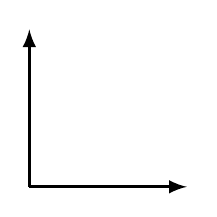
\begin{tikzpicture}
        \draw[-latex, very thick] (0, 0) -- (2, 0);
        \draw[-latex, very thick] (0, 0) -- (0, 2);
    \end{tikzpicture}
    
    \caption{Visualization of uniform convergence. If $f_n \rightarrow f$, uniformly, for any $\e > 0$, we can find $N$ such that for $n \geq N$, $f_n(x)$ lies in the $\e$-tube around $f$.}
    \label{fig40}
\end{figure}

\begin{nexample}{}{}
    
\end{nexample}

\begin{nexample}{}{}
    
\end{nexample}

\begin{theorem}{Cauchy Criterion for Uniform Convergence}{7.8}
    
\end{theorem}
\begin{nproof}
    
\end{nproof}

\begin{theorem}{}{7.9}
    
\end{theorem}
\begin{nproof}
    
\end{nproof}

\begin{ndef}{: Uniform Convergence of Series}{}
    
\end{ndef}

\begin{theorem}{Weierstrauss M-Test}{7.10}
    
\end{theorem}
\begin{nproof}
    
\end{nproof}

\subsection{Uniform Convergence and Integration}

\subsection{Uniform Convergence and Differentiation}

\subsection{Equicontinuituous Families of Functions}

\subsection{The Stone-Weierstrauss Theorem}


\section[Some Special Functions]{\hyperlink{toc}{Some Special Functions}}

\subsection{Power Series, Revisited}
Recall our definition of power series (Definition \ref{def:3.38}), functions of the form:
\begin{align*}
    f(x) = \sum_{n=0}^\infty c_n x^n.
\end{align*}
Also recall the radius of convergence (Theorem \ref{thm:3.39}) of such power series, defined as:
\begin{align*}
    R = \frac{1}{\limsup_{n \rightarrow \infty}\sqrt[n]{\abs{c_n}}}.
\end{align*}
Note that if $\limsup_{n \rightarrow \infty}\sqrt[n]{\abs{c_n}} = \infty$, then $R = 0$, and if $\limsup_{n \rightarrow \infty}\sqrt[n]{\abs{c_n}} = 0$, then $R = \infty$. The series converges absolutely for $\abs{x} < R$ and diverges for $\abs{x} > R$.

\begin{figure}[htbp]
    \centering
    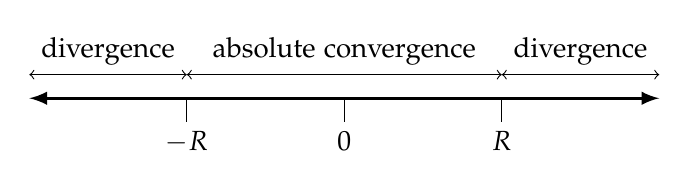
\begin{tikzpicture}[scale=2]
        \draw[latex-latex, very thick] (-2, 0) -- (2, 0);
        \draw[] (0, 0) -- (0, -0.15);
        \draw[] (1, 0) -- (1, -0.15);
        \draw[] (-1, 0) -- (-1, -0.15);
        \node[below] at (0, -0.15) {$0$};
        \node[below] at (1, -0.15) {$R$};
        \node[below] at (-1, -0.15) {$-R$};
        \draw[<->] (1, 0.15) -- (-1, 0.15);
        \draw[<->] (1, 0.15) -- (2, 0.15);
        \draw[<->] (-1, 0.15) -- (-2, 0.15);
        \node[above] at (0, 0.15) {absolute convergence};
        \node[above] at (1.5, 0.15) {divergence};
        \node[above] at (-1.5, 0.15) {divergence};
    \end{tikzpicture}
    
    \caption{Visualization of the radius of convergence for $f(x) = \sum_{n=0}^\infty c_nx^n$, $x \in \RR$.}
    \label{fig49}
\end{figure}

\begin{theorem}{}{8.1}
    If $\sum_{n=0}^\infty c_nx^n$ converges for $\abs{x} < R$, let $f(x) = \sum_{n=0}^\infty c_n x^n$ for $\abs{x} < R$. Then, the series converges uniformly on $[-R + \e, R - \e]$ for any $\e > 0$, $f$ is differentiable (and hence continuous) on $(-R, R)$ and $f'(x) = \sum_{n=0}^\infty nc_nx^{n-1}$. 
\end{theorem}

\begin{nproof}
    We first show the uniform convergence on $[-R + \e, R - \e]$. For $\abs{x} \leq R - \e$, we have that $\abs{c_nx^n} \leq \abs{x_n}(R - \e)^n$. Since $\sum_n \abs{c_n}(R - \e)^n < \infty$ (by the assumed absolute convergence on $(-R, R)$), we have that $\sum_n c_nx^n$ converges uniformly in $\abs{x} \leq R - \e$ by the M-test (Theorem \ref{thm:7.10}).

    We next prove the claim about the differentiability/derivative of $f$. The radius of convergence of $\sum_n nc_n x^{n-1}$ is:
    \begin{align*}
        \frac{1}{\limsup_{n \rightarrow \infty}\sqrt[n]{\abs{nc_n}}} = \frac{1}{\limsup_{n \rightarrow \infty}\sqrt[n]{\abs{c_n}}} = R
    \end{align*}
    so since $f$ converges in $(-R, R)$, so does $\sum_n nc_nx^{n-1}$. Now, let $s_n(x) = \sum_{m=0}^n c_mx^m$. Then, by the linearity of the derivative we have that $s_n'(x) = \sum_{m=1}^n mc_mx^{m-1}$. By the first part of the proof, we have that $s_n'(x) \rightarrow \sum_{m=1}^\infty mc_mx^{m-1}$ uniformly on $[-R + \e, R - \e]$. Since $s_n(x) \rightarrow f(x)$ uniformly, by Theorem \ref{thm:7.17}, we have that $f'$ exists on $[-R +\e, R - \e]$ and $f'(x) = \sum_{m=1}^\infty mc_mx^{m-1}$. Since $\e$ is arbitrary, $f'$ exists and is equal to $\sum_{m=1}^\infty mc_mx^{m-1}$ for all $x \in (-R, R)$. \qed 
\end{nproof}
\noindent As a remark, note that we can (interestingly) prove the differentiability of $f$ on $(-R, R)$ from the uniform convergence on $[-R + \e, R - \e]$.

\begin{ncorollary}{}{}
    If $f(x) = \sum_{n=0}^\infty c_nx^n$ converges for $\abs{x} < R$, then $f^{(k)}(x)$ exists for all $k \in \NN$ and for all $x \in (-R, R)$. It is given by:
    \begin{align*}
        f^{(k)}(x) = \sum_{n=k}^\infty n(n-1)\ldots(n-k+1)c_nx^{n-k} \quad (*)
    \end{align*}
    and consequently, we have that $c_k = \frac{f^{(k)(0)}}{k!}$, so $f(x) = \sum_{n=0}^\infty \frac{f^{(n)}(0)}{n!}x^n$.
\end{ncorollary}
\noindent Compare the above Corollary to Taylor's theorem (Theorem \ref{thm:5.15}). Here, we take our taylor polynomial and extend it to an infinite series (the limit of polynomials). 

\begin{nproof}
    By Theorem \ref{thm:8.1}, we have that $f'(x) = \sum_{n=1}^\infty nc_nx^{n-1}$ and $f''(x) = \sum_{n=2}^\infty n(n-1)c_nx^{n-2}$ and so on. Setting $x = 0$ in $(*)$, we have that $f^{(k)}(0) = n(n-1)\ldots 1 c_n = n! c_k$, so $c_n = \frac{f^{(k)}(0)}{n!}$. \qed
\end{nproof}
\noindent Recall the definition of \emph{analytic functions}, which are infinite differentiable and can be represented as sums or series of derivatives evaluated at zero. 

\begin{nexample}{}{}
    As we discussed in Chapter 5, there are infinitely differentiable functions that are not analytic. Let:
    \begin{align*}
        f(x) = \begin{cases}
            \exp(-\frac{1}{x^2}) & x \neq 0
            \\ 0 & x = 0
        \end{cases}
    \end{align*}
    By Theorem \ref{thm:8.1}, $f$ is infinitely differentiable, and $f^{(n)}(0) = 0$ for all $n \in \NN$. But, $f(x) \neq 0$ except at $x = 0$. Hence, $f(x) \neq \sum_{n=0}^\infty \frac{f^{(n)}(0)}{n!}x^n$ except at $x = 0$. This is true despite the fact that the RHS converges to zero for all $x \in \RR$. 
\end{nexample}

\begin{nexample}{}{}
    Bump functions are continuous, infinitely differentiable functions of compact support (it is zero outside of a compact set). For example, 
    \begin{align*}
        f(x) = \begin{cases}
            \exp(-\frac{1}{1-x^2}) & x \in (-1, 1)
            \\ 0 & \abs{x} \geq 1
        \end{cases}
    \end{align*}
    is an example of a bump function. Such functions are very useful in the study of functional analysis and PDEs.
\end{nexample}
\begin{figure}[htbp]
    \centering
    \begin{tikzpicture}[scale=1.5]
        \draw[-latex] (0, 0) -- (0, 2);
        \draw[latex-latex] (-2, 0) -- (2, 0);
        \draw[blue, thick, smooth, samples = 100, domain=-0.999:0.999, variable = \x] plot(\x, {3*exp(-1/(1-(\x)*(\x)))});
        \draw[->, blue, thick] (1, 0) -- (1.95, 0);
        \draw[->, blue, thick] (-1, 0) -- (-1.95, 0);
        \draw[] (1, 0) -- (1, -0.15);
        \draw[] (-1, 0) -- (-1, -0.15);
        \node[below] at (1, -0.15) {$1$};
        \node[below] at (-1, -0.15) {$-1$};
        \node[right] at (0, 1.23) {$e^{-1}$};
    \end{tikzpicture}
    
    \caption{Plot of the bump function $f$ from the above example.}
    \label{fig50}
\end{figure}

\subsection{The Exponential Function}

\subsection{The Logarithm}

\subsection{Sine and Cosine}

\subsection{Fourier Series}
\section{Functions of Several Variables}

\end{document}